\documentclass[
	oneside,         	 %% Comente essa linha para imprimir frente e verso
	pagestart=firstchapter,
%	english,
%	french,
%	spanish,
	brazil	        %% Idioma principal 
]{abntbibufjf}


\cftsetindents{figure}{0em}{4.6em}
\renewcommand*{\cftfigureaftersnum}{\hfill \textendash \space \space} 
%%\renewcommand*{\cftfigureaftersnum}{\space \textendash \space} 

%\newcommand{\quadroname}{Quadro}
%\newfloat[chapter]{quadro}{lof}{\quadroname}
%\newlistentry{quadro}{lof}{0}
%\cftsetindents{quadro}{0em}{4.2em}
%\setfloatadjustment{quadro}{\centering}
%\counterwithout{quadro}{chapter}
%\renewcommand{\cftquadroname}{\quadroname\space} 
%\renewcommand*{\cftquadroaftersnum}{\hfill \textendash \space} 
%\renewcommand{\cftquadroafterpnum}{\cftparfillskip}
%\setfloatlocations{quadro}{hbtp} 

\newcommand{\fotografianame}{Fotografia}
\newfloat[chapter]{fotografia}{lof}{\fotografianame}
\newlistentry{fotografia}{toc}{0}
\cftsetindents{fotografia}{0em}{3.1em}
\setfloatadjustment{fotografia}{\centering}
\counterwithout{fotografia}{chapter}
\renewcommand{\cftfotografianame}{\fotografianame\space} 
\renewcommand*{\cftfotografiaaftersnum}{\hfill \textendash \space \space} 
\renewcommand{\cftfotografiaafterpnum}{\cftparfillskip}
\setfloatlocations{fotografia}{hbtp}

\newcommand{\diagramaname}{Diagrama}
\newfloat[chapter]{diagrama}{lof}{\diagramaname}
\newlistentry{diagrama}{toc}{0}
\cftsetindents{diagrama}{0em}{3.3em}
\setfloatadjustment{diagrama}{\centering}
\counterwithout{diagrama}{chapter}
\renewcommand{\cftdiagramaname}{\diagramaname\space} 
\renewcommand*{\cftdiagramaaftersnum}{\hfill \textendash \space \space} 
\renewcommand{\cftdiagramaafterpnum}{\cftparfillskip}
\setfloatlocations{diagrama}{hbtp}

\newcommand{\fluxogramaname}{Fluxograma}
\newfloat[chapter]{fluxograma}{lof}{\fluxogramaname}
\newlistentry{fluxograma}{lof}{0}
\cftsetindents{diagrama}{0em}{3.3em}
\setfloatadjustment{fluxograma}{\centering}
\counterwithout{fluxograma}{chapter}
\renewcommand{\cftfluxogramaname}{\fluxogramaname\space} 
\renewcommand*{\cftfluxogramaaftersnum}{\hfill \textendash \space \space} 
\renewcommand{\cftfluxogramaafterpnum}{\cftparfillskip}
\setfloatlocations{fluxograma}{hbtp}


\pdfminorversion=7				%% Retira Warning "pdflatex.exe PDF inclusion: found PDF version <1.7>, but at most version <1.5> allowed"

% formatação
\usepackage{lmodern}
\usepackage[T1]{fontenc}
\usepackage[utf8]{inputenc}
\usepackage{indentfirst}
\usepackage{setspace}
\usepackage{url}
\usepackage{pdfpages} % Para adicionar folha de pdf
\usepackage{lastpage}


\usepackage{graphicx}
\usepackage{color}
\usepackage{microtype}
\usepackage{textcomp}


%--Pacotes Adicionados----------------------------

% pacote matemático
\usepackage{amsmath}                %pacote matemático da American Mathematical Society.
\usepackage{amsfonts}
\usepackage{amssymb}
\usepackage{amstext}
\usepackage{mathrsfs}               %pacote para fontes usadas em transformadas.
\usepackage[brazil]{babel}
\usepackage{xfrac}
\usepackage{icomma}                %notação decimal com virgula.
\usepackage{bm}                     %bold math
\DeclareMathOperator{\sen}{sen}     %declara operador seno.
%tabelas
\usepackage{multirow}
\usepackage{booktabs}
\usepackage{makecell} %espaçamento entre linhas
\usepackage{longtable}%quebra de tabela entre páginas
% \usepackage{array}
%figura
% \usepackage[caption=false,font=normalsize]{subfig} 
% \captionsetup[figure]{position=top}
% \captionsetup[subfigure]{position=bottom}
\usepackage{pdflscape}			%Colocar a figura em paisagem
\usepackage{rotating}			%rotacionar a figura e a legenda
\usepackage{float}
\usepackage{graphicx}
\usepackage{subcaption}
%\newcommand{\subfigureautorefname}{\figureautorefname}		%Utilizar o autoref
\usepackage{csquotes}
% listas
\usepackage{glossaries}
\usepackage[printonlyused]{acronym} 		%Para criar lista de acrônimos
%\usepackage[nolist,nohyperlinks]{acronym}	%Para criar lista de acrônimos sem lista
\usepackage{siunitx}			%Coloca no sistema de unidades internacional

% bibliografia
\usepackage[alf,abnt-emphasize=bf,abnt-etal-list=0, abnt-etal-text=it,abnt-etal-cite=3]{abntex2cite}	%% Citação mais arcaica, mas considerada como única aceitável para algumas institições
\usepackage{url6023}		%Consertar o <> devido a atualização da norma ABNT 6023

% citações e listas
\usepackage{verbatim}

\usepackage{url}


%-----------------------------------------------------------------------------

%% Obs.: Alguns acentos foram omitidos.

\titulo{Análise da Viabilidade do Fluxo de Potência com Multiplicador Ótimo: uma abordagem considerando os Fractais de Newton-Raphson}
%\subtitulo{Digite o subtítulo do trabalho, somente os nomes próprios com letras iniciais maiúsculas} 

\autor{Gabriel Halfeld Limp de Carvalho}
\autorR{Halfeld Limp de Carvalho, Gabriel}

\local{Juiz de Fora} %%Digitar o nome da cidade
\dia{27} %%Digitar o dia da defesa
\mes{Junho} %%Escrever por extenso o mês da defesa
\ano{2024} %%Digitar o ano da defesa

\orientador[Orientador:]{Igor Delgado de Melo} %%Se precisar, troque [Orientador:] por [Orientadora:]
\orientadorR{Delgado de Melo, Igor} 
\orientadorTitulo{Prof.} %%Digitar, dentro de chaves {}, a titula\c{c}\~ao do(a) orientador(a). Por exemplo: Prof., Eng.
\orientadorDegree{Dr.} %%Digitar, dentro das chaves {}, grau do(a) orientador(a). Por exemplo: Ph.D., D.Sc., Dr.

% \coorientador[Coorientador:]{} %% Comentar esta linha se nao tiver coorientador. Se precisar, troque por [Cooorientadora:]. 
% \coorientadorR{} %% Comentar esta linha se n\~ao tiver coorientador.
% % \coorientadorTitulo{Prof.} %% Comentar esta linha se n\~ao tiver coorientador.
% \coorientadorDegree{} %% Comentar esta linha se n\~ao tiver coorientador.

\instituicao{Universidade Federal de Juiz de Fora}
\faculdade{Faculdade de Engenharia} %%Digitar, dentro das chaves {}, o nome da faculdade ou do instituto.

\area{Sistemas de Potência} %%Digitar, dentro das chaves {}, a área ou modalidade do curso.

\tipodocumento{1} %% Digitar 1, 2 ou 3 dentro das { }: 1-> TCC; 2-> Mestrado; 3-> Doutorado

\ifthenelse{\equal{\inseretipodocumento}{1}}
	{\programa{Coordenação do Curso de Engenharia Elétrica}}
	{\programa{Programa de Pós-Graduação em Engenharia Elétrica}}

\ifthenelse{\equal{\inseretipodocumento}{1}}
	{\objeto{Trabalho de Conclusão de Curso (Graduação)}}
	{\ifthenelse{\equal{\inseretipodocumento}{2}}
	{\objeto{Dissertação (Mestrado)}}
	{\objeto{Tese (Doutorado)}}
	}

\ifthenelse{\equal{\inseretipodocumento}{1}}
	{\natureza{Trabalho de Conclusão de Curso apresentado à \insereprograma ~da \insereinstituicao ~como requisito parcial à obtenção do grau de Bacharel em Engenharia Elétrica. Modalidade: \inserearea.}}
	{\ifthenelse{\equal{\inseretipodocumento}{2}}
	{\natureza{Dissertação apresentada ao \insereprograma ~da \insereinstituicao ~como requisito parcial à obtenção do título de Mestre em Engenharia Elétrica. Área: \inserearea.}}
	{\natureza{Tese apresentada ao \insereprograma ~da \insereinstituicao ~como requisito parcial à obtenção do título de Doutor em Engenharia Elétrica. Área: \inserearea.}}
	}

%% Abaixo, prencher com os dados da parte final da ficha catalografica

\keywordI{Newton-Rapshon} %% Digitar, dentro das { }, a primeira palavra-chave.
\keywordII{Fluxo de Potência Continuado} %% Digitar, dentro das { }, a segunda palavra-chave.
\keywordIII{Fluxo de Potência Holomórfico} %% Digitar, dentro das { }, a terceira palavra-chave.

\finalcatalog{1. \inserekeywordI. 2. \inserekeywordII. 3. \inserekeywordIII. I. \insereorientadorR , orient. II. Título.}
\ifnotempty{\inserecoorientador}{
	\finalcatalog{1. \inserekeywordI. 2. \inserekeywordII. 3. \inserekeywordIII. I. \insereorientadorR, orient. II. \inserecoorientadorR, coorient. III. Título.}}


\begin{document}

%% ELEMENTOS PRÉ-TEXTUAIS

%% Capa
\inserecapa

%% Folha de rosto
\inserefolhaderosto

%% Ficha catalográfica. AO IMPRIMIR, DEIXAR NO VERSO DA FOLHA DE ROSTO.
\inserecatalog  


%% Folha de aprovacao
%\includepdf{./Folha_Aprovacao.pdf}
\begin{folhadeaprovacao}
	\inicfolhaaprov
	
	Aprovada em \inseredia~de \inseremes~de \insereano. %%Preencher com a data 
	
	\vfill
	\begin{center} BANCA EXAMINADORA \end{center}
	\assinatura{\insereorientadorTitulo~\insereorientador, \insereorientadorDegree \ - Orientador \\ Universidade Federal de Juiz de Fora - UFJF}  %%Orientadora
	{\ifnotempty{\inserecoorientador}{%
			{\assinatura{\inserecoorientadorTitulo~\inserecoorientador, \inserecoorientadorDegree \ - Coorientador \\ Universidade Federal de Juiz de Fora - UFJF} \par }%
		}
	}
	\assinatura{Prof. Abilio Manuel Variz, D.Eng.\\ Universidade Federal de Juiz de Fora - UFJF}
	\assinatura{Candida Aparecida Delgado Meneghin, M.Eng.\\ Universidade Federal de Juiz de Fora - UFJF}
	%% Descomentar as próximas linhas no caso de mais membros na banca examinadora
%	\assinatura{Prof. Nome completo do terceiro examinador, Título\\ Nome da Instituição por extenso - SIGLA}
%	\assinatura{Prof. Nome completo do quarto examinador, Título\\ Nome da Instituição por extenso - SIGLA}
%	\assinatura{Prof. Nome completo do quinto examinador, Título\\ Nome da Instituição por extenso - SIGLA}
\end{folhadeaprovacao}
\cleardoublepage 


%% Dedicatoria. OPCIONAL. Colocar ``%'' no início da próxima linha, caso não queira.
\begin{dedicatoria} 
  \textit{\enquote{O que sabemos é uma gota, o que ignoramos é um oceano.}}
  
  (Isaac Newton)%% substituir 
\end{dedicatoria}

%% Agradecimentos. OPCIONAL. CASO SEJA BOLSISTA, INSERIR OS DEVIDOS AGRADECIMENTOS.
\begin{agradecimentos}

Agradeço aos meus pais, Esmeralda e Ricardo, por todo incentivo e apoio na minha jornada acadêmica. Ter pais que compreendem como a educação é importante para a formação de um cidadão foi essencial para que eu tenha chegado até aqui.


Quero agradecer à minha querida namorada, Sara, pelo companheirismo e constante apoio. Ao seu lado, encontro fé nos dias difíceis e compartilho minhas maiores alegrias nos momentos de felicidade. Dedico este trabalho a você com todo carinho, pois sua presença foi fundamental para a sua conclusão.

Obrigado a Universidade Federal de Juiz de Fora e todo aquele que trabalhe para engrandecê-la, por proporcionar uma educação de qualidade para as pessoas. Sou privilegiado por fazer parte desta instituição que se destaca pelo compromisso com o ensino superior público e pela excelência acadêmica em diversas áreas do conhecimento.

Ao professor Igor Delgado, expresso minha gratidão pelos ensinamentos e pela confiança demonstradas ao longo da minha formação, desde a sala de aula até os desafios da iniciação científica e, agora, na orientação deste trabalho.

Agradeço aos membros da banca avaliadora, pela disponibilidade de participar e pelas contribuições dadas neste texto.

Por fim, quero agradecer a todas as pessoas que me acompanharam e contribuíram positivamente, de forma indireta, nessa trajetória.

\end{agradecimentos}

%% Ep\'igrafe. OPCIONAL. Colocar ``%'' no início da próxima linha, caso não queira.
%\begin{epigrafe} 
	``\textit{O que sabemos é uma gota; o que ignoramos é um oceano.}''\\
	(Isaac Newton).
\end{epigrafe}


%% Resumo em Português. OBRIGATÓRIO.
\begin{resumo}

Este trabalho apresenta uma análise sobre uma modificação do Fluxo de Potência em regime permanente utilizando o método de Newton-Raphson, o Fluxo de Potência com Multiplicador Ótimo, através da comparação com a formulação em coordenadas polares e retangulares. 

A pesquisa envolve a demonstração teórica dos métodos, bem como a implementação e testes em sistemas conhecidos na literatura: o IEEE 14 Barras, de transmissão, e o IEEE 33 Barras, de distribuição. A comparação da robustez de cada código é feita em três diferentes aspectos: tempo computacional, máximo carregamento e análise dos fractais de Newton-Raphson para cada sistema, visando compreender as vantagens e desvantagens da metodologia proposta.

O estudo indicou que o Fluxo de Potência com Multiplicador Ótimo, por mais que tenha exigido um maior tempo computacional e uma diferença irrisória na capacidade de convergir casos muito carregados, esse foi capaz de melhorar a convergência para uma maior faixa de palpites iniciais para as variáveis do problema em questão.


\textbf{Palavras-chave}: Fluxo de potência; Fractais; Newton-Raphson; Otimização; Sistemas de potência.
%%finalizadas por ponto e inicializadas por letra maiuscula.
\end{resumo}


%% Resumo em Inglês. OBRIGATÓRIO para teses e dissertações
\begin{otherlanguage*}{english}
\begin{resumo}[\textbf{ABSTRACT}]
This work presents an analysis of a modification of the Newton-Raphson method for Power Flow computation, namely the Optimal Power Flow (OPF), through comparison with formulations in polar and rectangular coordinates.

The research includes theoretical demonstrations of the methods as well as their implementation and testing on well-known systems in the literature: the IEEE 14-Bus transmission system and the IEEE 33-Bus distribution system. The robustness of each algorithm is compared in three different aspects: computational time, maximum loading, and analysis of Newton-Raphson fractals for each system, aiming to understand the advantages and disadvantages of the proposed methodology.

The study indicated that the Power Flow with Optimal Multiplier, despite requiring more computational time and showing a negligible difference in the ability to converge heavily loaded cases, was able to improve convergence for a wider range of initial guesses for the problem's variables.

\textbf{Keywords}: Fractals; Newton-Raphson; Optimization; Power flow; Power Systems. 
\end{resumo}
\end{otherlanguage*}


%% Lista de ilustra\c{c}\~oes. OPCIONAL. 
\pdfbookmark[0]{\listfigurename}{lof}  
\listoffigures*
\cleardoublepage

%% Lista de tabelas. OPCIONAL. 
\pdfbookmark[0]{\listtablename}{lot}
\listoftables*    %Coloque ``%'' no in\'icio desta linha, caso n\~ao queira lista de tabelas.
\cleardoublepage

\chapter*{\textbf{LISTA DE ABREVIATURAS E SIGLAS}}
\begin{acronym}[PRODIST] %% Depois de rodar a primeira vez, digite entre os [ ] a sigla mais longa para justificar a lista de acrônimos à esquerda
   \itemsep0em
    \acro{2D}{Duas Dimensões}
    \acro{ANEEL}{Agência Nacional de Energia Elétrica}
    \acro{B}{Susceptância}
    \acro{CCEE}{Câmara de Comercialização de Energia Elétrica}
    \acro{CA}{Corrente Alternada}
    \acro{CC}{Corrente Contínua}
    \acro{EPE}{Empresa de Pesquisa Energética}
    \acro{EBP}{Equações de Balanço de Potência}
    \acro{FACTS}{Sistema de Transmissão CA Flexível}
    \acro{FP}{Fluxo de Potência}
    \acro{FPC}{Fluxo de Potência Continuado}
    \acro{FPO}{Fluxo de Potência Ótimo}
    \acro{FPMO}{Fluxo de Potência com Multiplicador Ótimo}
    \acro{FPPOL}{Fluxo de Potência em Coordenadas Polares}
    \acro{FPRET}{Fluxo de Potência em Coordenadas Retangulares}
    \acro{FPORS}{Fluxo de Potência Ótimo com Restrições de Segurança}
    \acro{FOB}{Função Objetivo}
    \acro{GS}{Gauss-Seidel}
    \acro{G}{Condutância}
    \acro{IEEE}{Institute of Electrical and Electronics Engineers}
    \acro{N}{Número de Barras do Sistema}
    \acro{NPQ}{Número de Barras PQ}
    \acro{NPV}{Número de Barras PV}
    \acro{NR}{Newton-Raphson}
    \acro{ONS}{Operador Nacional do Sistema}
    \acro{PMC}{Ponto de Máximo Carregamento}
    \acro{PQ}{Barra de Carga}
    \acro{PRODIST}{Procedimentos de Distribuição de Energia Elétrica}
    \acro{PV}{Barra de Geração}
    \acro{R}{Resistência}
    \acro{SEP}{Sistema Elétrico de Potência}
    \acrodefplural{SEP}{Sistemas Elétricos de Potência}
    \acro{SIN}{Sistema Interligado Nacional}
    \acro{p.u.}{Por Unidade}
    \acro{UFJF}{Universidade Federal de Juiz de Fora}
    \acro{X}{Reatância indutiva}
\end{acronym}

% % % Lista de s\'imbolos. OPCIONAL

% \begin{simbolos} %%ALTERAR OS EXEMPLOS ABAIXO, CONFORME A NECESSIDADE

% \end{simbolos}





 
%% Sum\'ario
\pdfbookmark[0]{\contentsname}{toc}
\tableofcontents*
\cleardoublepage

%% ELEMENTOS TEXTUAIS
\textual

\acresetall

\chapter{INTRODUÇÃO}\label{cap:intro}
Este capítulo aborda, de forma concisa, o contexto subjacente a este trabalho. Em seguida, são meticulosamente abordadas as motivações e objetivos que moldaram a concepção deste estudo. Por fim, uma visão abrangente da estrutura deste documento é oferecida, destacando o conteúdo dos capítulos subsequentes.

\section{CONTEXTUALIZAÇÃO}
O estudo do \ac{FP} é fundamental para a operação, planejamento e expansão de \acp{SEP}. Através da análise dessa ferramenta, é possível obter informações valiosas sobre o comportamento do sistemas de diferentes escalas e cenários de operação, permitindo identificar pontos sensíveis, sobrecargas, perdas de potência e outros problemas que podem afetar a confiabilidade e a qualidade do fornecimento de energia elétrica. 

Com o crescimento da demanda por eletricidade e a expansão das redes de transmissão, ao longo do século XX e XXI, o estudo do fluxo de potência evoluiu para uma disciplina altamente especializada. O desenvolvimento de técnicas avançadas, como o método de \ac{NR}, permitiu aos engenheiros modelarem e otimizarem \acp{SEP} de larga escala, levando a melhorias significativas na eficiência e confiabilidade da rede elétrica. 


Atualmente, os \ac{SEP} enfrentam grandes desafios devido à sua expansão, impactos das mudanças climáticas, crescente uso de fontes intermitentes como solar e eólica, entre outros \cite{EPE_transmissao_desafios}. Pesquisas direcionadas a melhorar o desempenho dos estudos de \ac{FP} são necessárias. O intuito é se adaptar aos desafios atuais e lidar com sistemas mal condicionados e com alta variabilidade. "A análise do fluxo de potência no atendimento das cargas pressupõe a disponibilidade de ferramentas adequadas e confiáveis, principalmente quando o sistema
envolvido é de grande porte"(ZANETTA, 2006, p. 239).


\section{MOTIVAÇÃO}
Desde a década de 1950, quando os primeiros artigos técnicos sobre algoritmos de solução do \ac{FP} foram publicados, muitos métodos iterativos foram desenvolvidos. A maioria desses métodos é baseada em duas técnicas principais amplamente usadas na indústria atualmente: \ac{GS} e Newton-Raphson (\ac{NR}), sendo o último a técnica mais utilizada nos softwares comerciais atualmente \cite{IEEE_standard}.

A expressão sistemas "mal condicionados" refere-se à situação em que pequenas mudanças nos parâmetros do sistema de potência resultam em grandes mudanças nas soluções do problema \cite{11busSystem}. O problema de \ac{FP} utilizando métodos iterativos pode divergir por diversos motivos, principalmente por:
\begin{itemize}
    \item Proximidade ao \ac{PMC} do \ac{SEP};
    \item Estimativa inicial das variáveis de estado muito longe da solução real;
    \item Não existência de solução possível através do método computacional utilizado.
\end{itemize}

A partir disso, pode-se utilizar o conceito de regiões de segurança \cite{Overbye}, como na Figura \ref{fig:regiões de solução}, em que algumas regiões são definidas:

\begin{figure}[htpb!]
    \centering
    \caption{Regiões de Segurança do \ac{FP}}
    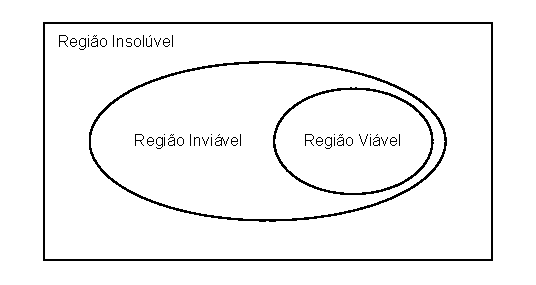
\includegraphics[scale=1.7]{textuais/capitulo1/figuras/regioes_seguranca.pdf}
    \label{fig:regiões de solução}
    \caption*{Fonte: Adaptada de Overbye (\citeyear{Overbye})}
\end{figure}


\begin{itemize}
    \item Região Viável: Região onde há solução para o problema que não viole os limites operacionais dos componentes do sistema;
    \item Região Inviável: Região onde há solução para o problema que viole um ou mais limites operacionais;
    \item Região Insolúvel: Região onde não há solução para o problema, onde provavelmente operar nessas condições geraria uma instabilidade que culminaria no colapso de tensão do sistema.
\end{itemize}

Estender a fronteira entre a região inviável e insolúvel oferece diversos benefícios principalmente no estudo de planejamento da expansão do \ac{SEP} e análise de contingências. Obter uma solução, mesmo inviável, pode facilitar estimativas de futuros projetos capazes de enfrentar um aumento de carga planejado, por exemplo.

Este estudo tem como motivação testar e analisar um método proposto por Iwamoto (1981)  que visa otimizar a atualização das variáveis de estado dentro do método de \ac{NR} e compará-lo com os métodos tradicionais em coordenadas polares e retangulares, visando explorar sua implementação. Isso envolve a análise teórica, o desenvolvimento de algoritmos computacionais e a realização de estudos de caso em sistemas de teste representativos.

\section{OBJETIVOS}
O objetivo deste trabalho consiste em fazer uma revisão bibliográfica acerca do método conhecido na literatura como Fluxo de Potência com Multiplicar Ótimo. Para isso, o trabalho foi dividido nas seguintes etapas:
\begin{itemize}
    \item Implementar o \ac{FPPOL} e \ac{FPRET};
    \item Implementar o \ac{FPMO};
    \item Testar e comparar os algoritmos em sistemas teste;
    \item Avaliar a utilização do método proposto explorando sistemas extremamente carregados, mapas fractais das múltiplas soluções do fluxo de potência e tempo computacional.
\end{itemize}

\section{ESTRUTURA DO DOCUMENTO}
A divisão deste trabalho é feita em cinco capítulos. O primeiro, de introdução, visa contextualizar e justificar ao leitor a necessidade da atual pesquisa, bem como definir os objetivos e a metodologia utilizada para o trabalho.

No capítulo 2, é feita uma revisão dos conceitos principais do \ac{FP} necessários para a compreensão adequada do tema, apresentando todo o desenvolvimento matemático, desde as séries de Taylor, até a formulação do método de \ac{NR} para ambos os sistemas de coordenadas retangulares e polares.

O capítulo 3 é composto pela formulação matemática completa do \ac{FPMO}, visando resolver os principais problemas encontrados ao tentar implementar o algoritmo.

O capítulo 4 será composto pelos resultados das simulações realizadas em sistemas teste, que servirão de apoio para as comparações dos métodos analisados.

Por último, o capítulo 5 engloba as conclusões finais alcançadas com o trabalho, somado de um futuro direcionamento para pesquisas posteriores.


\chapter{FUNDAMENTAÇÃO TEÓRICA}\label{cap:cap2}

\section{SÉRIES DE TAYLOR}
A expansão em séries de Taylor é uma ferramenta importante na matemática que permite aproximar uma função 
$f(x)$
desconhecida ou complicada por meio de um polinômio. Para isso, ela deve ser suficientemente suave, contínua e diferenciável \cite{Guidorizzi}.
A série é construída a partir das derivadas da função em um ponto específico 
$x_0$
, chamado ponto de expansão.

A forma geral é dada pela equação \eqref{eq:taylor_geral}:
\begin{equation}\label{eq:taylor_geral}
    f(x) = f(x_0) + f'(x_0)(x-x_0) + \frac{1}{2!}f''(x_0)(x-x_0)^2 +\dotsb+ \frac{1}{n!}f^{n}(x_0)(x-x_0)^n + \dotsb
\end{equation}

Vale ressaltar que a expansão se aproxima cada vez mais da função original conforme a série é truncada com um maior número de termos \cite{atkinson1989introduction}.
Pode-se, ainda, usar o teorema do erro de Taylor e ter uma estimativa do erro entre a função original em um ponto $b$,  e sua aproximação polinomial truncada no termo $n$ e avaliada em um ponto de expansão $x_0$, conforme a equação \eqref{taylor_erro}.
\begin{equation}\label{taylor_erro}
    E(b) = \frac{f^{n+1}(b)}{(n+1)!}(x-x_0)^{n+1}
\end{equation}

Para uma função multivariada $f(X)$ em que $X= [x_1,x_2,\cdots,x_k]^T$
, a expansão de Taylor até a segunda ordem é dada por \eqref{eq:taylor_multivariavel}.
\begin{equation}\label{eq:taylor_multivariavel}
f(X) \approx  f(X_0) + \nabla f(X_0).(X-X_0) + \frac{1}{2!} (X-X_0) H(X_0) (X-X_0)^T
\end{equation}

Onde o gradiente de $f$ avaliado em $X_0$ é dado por \eqref{eq:gradiente}.
\begin{equation}\label{eq:gradiente}
    \nabla f(X_0) = 
    \left.
    \begin{bmatrix}
        \frac{\partial f}{\partial x_1} \\
        \vdots \\
        \frac{\partial f}{\partial x_k}
    \end{bmatrix}
    \right|_{\substack X = X_0}
\end{equation}

E a matriz Hessiana $H$ avaliada em $X_0$ é obtida através de \eqref{eq:hessian_matrix}.
\begin{equation}\label{eq:hessian_matrix}
    H(X_0) = 
    \left.
\begin{bmatrix}
\frac{\partial^2 f}{\partial x_1^2} & \frac{\partial^2 f}{\partial x_1 \partial x_2} & \cdots & \frac{\partial^2 f}{\partial x_1 \partial x_k} \\
\frac{\partial^2 f}{\partial x_2 \partial x_1} & \frac{\partial^2 f}{\partial x_2^2} & \cdots & \frac{\partial^2 f}{\partial x_2 \partial x_k} \\
\vdots & \vdots & \ddots \\
\frac{\partial^2 f}{\partial x_k \partial x_1} & \frac{\partial^2 f}{\partial x_k \partial x_2} & \cdots & \frac{\partial^2 f}{\partial x_k^2} \\
\end{bmatrix} 
\right|_{\substack X = X_0}
\end{equation}

De acordo com Tinney et al. (\citeyear{NewtonRaphson}), o método de Newton-Raphson pode ser aplicado para encontrar raízes de sistemas de equações não lineares
$F(X) = [f_1(X), f_2(X),\cdots,f_k(X)]^T$, que é o caso do problema do \acs{FP}.

A forma geral, truncada na segunda ordem, é apresentada pela equação \eqref{eq:sistema_multi_taylor}:
\begin{equation}\label{eq:sistema_multi_taylor}
    F(X) \approx F(X_0) + J(X_0)(X-X_0) + \frac{1}{2!}(X-X_0)^T H(X_0)(X-X_0)
\end{equation}

Onde $J(X_0)$ é a matriz Jacobiana avaliada em $X_0$, dada por \eqref{eq:Jacobiana_multi}:
\begin{equation}\label{eq:Jacobiana_multi}
    J(X_0)= 
    \left. 
    \begin{bmatrix}
    \frac{\partial f_1}{\partial x_1} & \cdots & \frac{\partial f_1}{\partial x_k} \\
    \vdots & \ddots & \vdots \\
    \frac{\partial f_k}{\partial x_1} & \cdots & \frac{\partial f_k}{\partial x_k} 
    \end{bmatrix}
    \right|_{\substack{X = X_0}}
\end{equation}

E $H(X_0)$ é o tensor Hessiano avaliado em $X_0$, dado por \eqref{eq:Hessian_tensor}:

\begin{equation}\label{eq:Hessian_tensor}
    H(X_0) = 
    \left. 
    \begin{bmatrix}
        \begin{bmatrix}
            \frac{\partial^2 f_1}{\partial x_1^2} & \frac{\partial^2 f_1}{\partial x_1 \partial x_2} & \cdots & \frac{\partial^2 f_1}{\partial x_1 \partial x_k} \\
            \frac{\partial^2 f_1}{\partial x_2 \partial x_1} & \frac{\partial^2 f_1}{\partial x_2^2} & \cdots & \frac{\partial^2 f_1}{\partial x_2 \partial x_k} \\
            \vdots & \vdots & \ddots \\
            \frac{\partial^2 f_1}{\partial x_k \partial x_1} & \frac{\partial^2 f_1}{\partial x_k \partial x_2} & \cdots & \frac{\partial^2 f_1}{\partial x_k^2} 
        \end{bmatrix}
        \\
        \\
        \begin{bmatrix}
            \frac{\partial^2 f_2}{\partial x_1^2} & \frac{\partial^2 f_2}{\partial x_1 \partial x_2} & \cdots & \frac{\partial^2 f_2}{\partial x_1 \partial x_k} \\
            \frac{\partial^2 f_2}{\partial x_2 \partial x_1} & \frac{\partial^2 f_2}{\partial x_2^2} & \cdots & \frac{\partial^2 f_2}{\partial x_2 \partial x_k} \\
            \vdots & \vdots & \ddots \\
            \frac{\partial^2 f_2}{\partial x_k \partial x_1} & \frac{\partial^2 f_2}{\partial x_k \partial x_2} & \cdots & \frac{\partial^2 f_2}{\partial x_k^2} 
        \end{bmatrix}
        \\
        \vdots
        \\
        \begin{bmatrix}
            \frac{\partial^2 f_k}{\partial x_1^2} & \frac{\partial^2 f_k}{\partial x_1 \partial x_2} & \cdots & \frac{\partial^2 f_k}{\partial x_1 \partial x_k} \\
            \frac{\partial^2 f_k}{\partial x_2 \partial x_1} & \frac{\partial^2 f_k}{\partial x_2^2} & \cdots & \frac{\partial^2 f_k}{\partial x_2 \partial x_k} \\
            \vdots & \vdots & \ddots \\
            \frac{\partial^2 f_k}{\partial x_k \partial x_1} & \frac{\partial^2 f_k}{\partial x_k \partial x_2} & \cdots & \frac{\partial^2 f_k}{\partial x_k^2}    
        \end{bmatrix}
    \end{bmatrix}
    \right|_{\substack{X = X_0}}
\end{equation}

\section{MÉTODO DE NEWTON RAPHSON}
Muitos sistemas físicos complexos são descritos por equações as quais não possuem uma solução analítica direta, por isso técnicas para obter uma solução numérica aproximada foram desenvolvidas \cite{Stagg}.
Desenvolvido no século XVII por Isaac Newton e Joseph Raphson, o método de Newton-Raphson (\acs{NR}) é um algoritmo que permite encontrar raízes de uma função desconhecida,  desde que se tenha acesso ao valor da função e sua derivada em diferentes pontos. 

Nessa seção, será apresentada a fundamentação teórica do método.
\subsection{Formulação}
O método de NR começa definindo-se uma aproximação inicial
$X_0$
para as raízes procuradas e utilizando essa aproximação como ponto de expansão da série de Taylor, que será truncada na primeira derivada, apresentado abaixo por \eqref{eq:taylor_NR_1}:

\begin{equation}\label{eq:taylor_NR_1}
    F(X) \approx F(X_0) + J(X_0)(X-X_0)
\end{equation}

Ou, por \eqref{eq:taylor_jacobiana}:
\begin{equation}\label{eq:taylor_jacobiana}
    F(X) \approx F(X_0) + J(X_0)\Delta X
\end{equation}

Onde, $\Delta X$ é chamado de incremento de $X$ e é dado por \eqref{eq:deltax}:

\begin{equation}\label{eq:deltax}
    \Delta X = X-X_0
\end{equation}

Como se deseja encontrar as raízes do sistema de equações 
$F(X)$
, iguala-se o lado esquerdo da equação \eqref{eq:taylor_jacobiana} a zero, obtendo-se o valor do incremento 
$\Delta X$, que será usado como ponto de expansão da série de Taylor da próxima iteração $n+1$, como mostram as equações \eqref{delta_x_2} \eqref{eq:atualização_x_0} e \eqref{eq:n=n+1}.

\begin{equation}\label{delta_x_2}
    \Delta X^{(n)} = [J(X_0^{(n)})]^{-1}.\,F(X_0^{(n)})
\end{equation}   

\begin{equation}\label{eq:atualização_x_0}
    X_0^{(n+1)} = X_0^{(n)} + \Delta X^{(n)}
\end{equation}

\begin{equation}\label{eq:n=n+1}
    n = n+1
\end{equation}

Novamente é calculado o valor de $F(X_0^{(n)})$ e avaliado se obedece um erro máximo aceitável
$\epsilon$. Se o erro for maior, mais uma iteração será feita e o processo se repete. Existem casos que o método não consegue encontrar raízes que obedeçam ao erro, por isso define-se um número máximo de iterações $n_{max}$ suficientemente grande para que, caso seja extrapolado, diz-se que o processo divergiu.

Na figura \ref{fig:diagrama_NR}, um fluxograma representativo do método de Newton-Raphson é apresentado, sendo dividido em blocos para sua explicação em detalhes:

\begin{itemize}
    \item Bloco 1: Início do método de Newton-Raphson;
    \item Bloco 2: Inicializa as variáveis de iterações $n$, do incremento $\Delta X$ e da estimativa inicial para as variáveis de estado $X_0$;
    \item Bloco 3: Calcula o valor da função no ponto de expansão $X_0$;
    \item Bloco 4: Avalia se o valor da função com a estimativa atual é menor ou maior ou igual que o erro máximo aceitável $\epsilon$;
    \item Bloco 5: Caso o valor da função não respeite $\epsilon$, atualiza-se o contador de iterações $n$;
    \item Bloco 6: Avalia se o contador de iterações extrapolou o número máximo de iterações $n_{max}$;
    \item Bloco 7: Calcula a Jacobiana avaliada em $X_0^{n-1}$;
    \item Bloco 8: Com a Jacobiana, calcula o incremento $\Delta X^{n-1}$;
    \item Bloco 9: Atualiza $X_0$ na iteração $n$ com o incremento calculado;
    \item Bloco 10: Caso o valor da função respeite $\epsilon$, o processo finaliza com convergência;
    \item Bloco 11: Caso o número de iterações extrapole o $n_{max}$, o processo se encerra sem uma raíz com erro máximo desejado, indicando divergência.
\end{itemize}

\begin{figure} [H]
    \centering
    \caption{Fluxograma do método Newton-Raphson}
    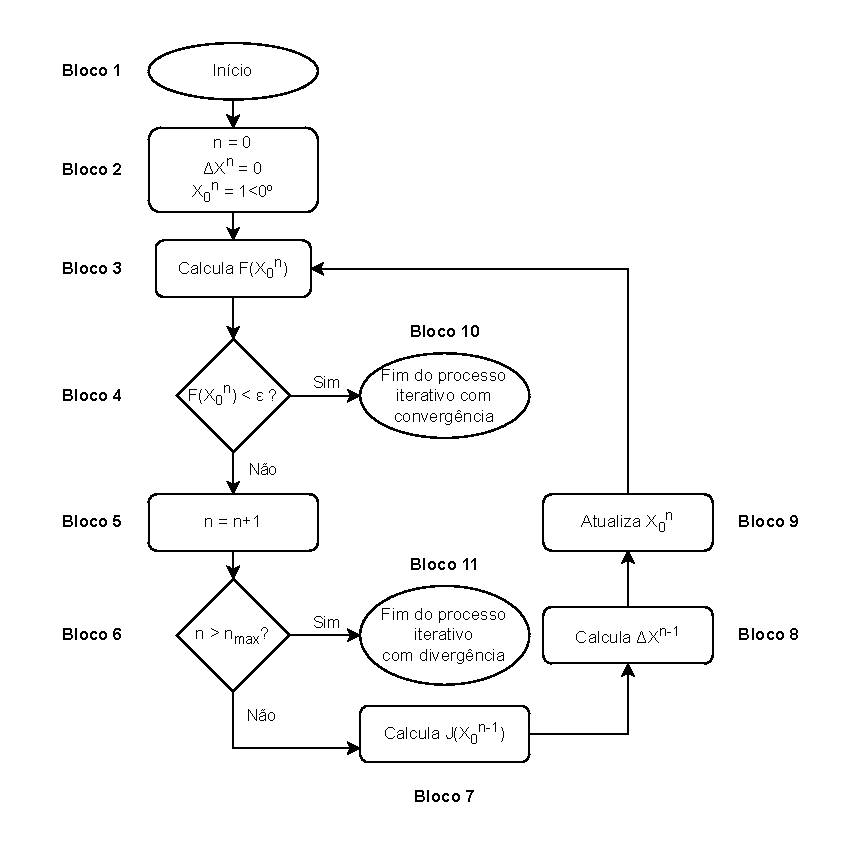
\includegraphics{textuais/capitulo2/figuras/Diagrama_NR_4.drawio.pdf}
    \caption*{Fonte: Elaborada pelo autor}
    \label{fig:diagrama_NR}
\end{figure}


\subsection{Características importantes do método}
O método de NR é altamente dependente do palpite inicial para o vetor de variáveis de estado $X$. Isso ocorre porque a série de Taylor truncada no primeiro termo só se comporta bem em regiões muito próximas da solução. 

Se 
$X_0$
for de fato próximo da solução, a diferença entre a solução atual e a solução verdadeira diminui quadraticamente a cada iteração, característica do método de Newton-Raphson \cite{NewtonRaphson}.

Porém, se 
$X_0$
for um valor muito distante da solução, o sistema pode divergir, levando a nenhuma solução ou a soluções sem sentido físico (soluções instáveis ou espúrias), mesmo que haja uma solução possível para o sistema.

Além disso, pode ser que o sistema de fato não possua solução. Isso também pode ser um problema, principalmente para estudos de planejamento da expansão de um sistema elétrico de grande porte.
Dependendo do caso, é necessário obter uma estimativa da solução, visando entender quais melhorias o sistema precisa para alcançar a convergência na região viável.

Finalmente, é possível que o método não encontre solução quando a matriz Jacobiana é singular ou muito próxima da singularidade. Nesses casos, a inversão de $J$ se torna indefinida, impedindo obter soluções para o problema.

Para combater esse problema de convergência, diversos métodos foram propostos na literatura como o Fluxo de Potência Continuado e outros métodos de otimização heurísticos, como Algoritmos Genéticos.

Um desses métodos é o método do Multiplicador Ótimo, que será visto aprofundadamente no Capítulo \ref{cap:cap3}.

\section{FLUXO DE POTÊNCIA USANDO NR}
O Fluxo de Potência é um procedimento essencial na análise de sistemas elétricos de potência, pois visa determinar o estado operativo da rede elétrica em regime permanente \cite{ONSsubmodulo2_3}. 

Em outras palavras, considerando as características das cargas a serem conectadas, os tipos de geradores, os limites de geração e os limites operativos das linhas, o objetivo principal é determinar:
\begin{itemize}
    \item Tensões nodais: magnitudes e ângulos das tensões em todas as barras (ou nós) do sistema;
    \item Potência reativa dos geradores;
    \item Fluxo de potência nas linhas: Avaliar se as linhas estão operando próximas de seus limites.
\end{itemize}

Nesta seção, será abordado como representar uma rede elétrica, os tipos de barras, as equações de potência e, finalmente, como utilizar o método NR para o problema.


\subsection{Matriz admitância nodal}
A matriz admitância nodal, ou matriz 
$Y_{barra}$
, desempenha um papel fundamental na análise de circuitos elétricos de potência, sendo uma representação matricial dos parâmetros do circuito. Sua importância reside no fato de que ela permite relacionar o vetor
$\Dot I$
de correntes injetadas nos nós
com o vetor
$\Dot V$
de tensões nodais do sistema, de acordo com \eqref{eq:I=YV}. Vale ressaltar que a formulação apresentada é válida apenas para representações monofásicas e sem mútuas \cite{Robba}.

É uma matriz quadrada e simétrica de ordem
$n \times n$
, em que 
$n$
é o número de nós do sistema.
\begin{equation} \label{eq:I=YV}
    \Dot I = Y \, \Dot V
\end{equation}

Uma vantagem de seu uso é que sua formação é simples e pode ser feita por inspeção visual do sistema:
\begin{itemize}
    \item Elementos diagonais “$Y_{kk}$”: Soma de todas as admitâncias conectadas ao nó "$k$";
    \item Elementos não diagonais "$Y_{km}$": Negativo da admitância equivalente entre o nó "$k$" e o nó "$m$".
\end{itemize}

Como o número de nós conectados a um nó específico é limitado em um \ac{SEP}, a 
${Y_{barra}}$
se torna uma matriz esparsa, aumentando seu grau de esparsidade quadraticamente conforme o número de barras aumenta em um sistema. Formas de lidar com essas matrizes computacionalmente, evitando armazenar muitos zeros já são uma realidade nos programas de \ac{FP} atuais, mas não serão tratados neste trabalho.

\subsection{Equações Algébricas do Fluxo de Potência}

As equações algébricas do \ac{FP} apresentadas são conhecidas na literatura por formulação por injeção de potência.
Baseado nas leis de Kirchoff, as potências ativas e reativas injetadas em uma barra $k$ podem ser determinadas através das equações \eqref{eq:PkQk_esp}, onde em termos práticos, a potência gerada $P_{gerada, k}$ e $Q_{gerada, k}$ é a potência fornecida por geradores conectados a barra $k$ e a potência demandada $P_{demandada, k}$ e $Q_{demandada, k}$ é a potência consumida por cargas conectadas a barra $k$.
\begin{equation} \label{eq:PkQk_esp}
    \begin{split}
        P_k &= P_{gerada,k} - P_{demandada,k} \\
        Q_k &= Q_{gerada,k} - Q_{demandada,k} 
    \end{split}
\end{equation}

Logo, a potência complexa injetada em uma barra $k$ pode ser definida em \eqref{eq:S_k} através das tensões e correntes nodais:
\begin{equation} \label{eq:S_k}
     S_k = P_k + j\,Q_k = \Dot V_k \, \Dot I_k^*
\end{equation}

É interessante observar que dessa forma, há 6 variáveis para cada barra: duas para parte real e imaginária da potência complexa, tensão complexa e corrente complexa. Por isso, o conjugado da corrente injetada $\Dot I_k$ será representado em termos da matriz admitância, de acordo com \eqref{eq:I_k^*}.
\begin{equation} \label{eq:I_k^*}
    \Dot I_k^* = (\sum_{m \in K} Y_{km}\, \Dot V_m)^* = \sum_{m \in K} Y_{km}^*\, \Dot V_m^* 
\end{equation}

Onde K representa o conjunto de barras ligadas a barra $k$.

O conjugado da matriz admitância nodal é facilmente obtido, basta separar a sua parte real, \ac{G}, da sua parte imaginária, \ac{B}, como em \eqref{eq:Y=G+jB}.
\begin{equation} \label{eq:Y=G+jB}
        Y^* = G - j\,B
\end{equation}

Além disso, a tensão $\Dot V_k$ e o conjugado da tensão $\Dot V_m$ podem ser escritos em coordenadas polares, de acordo com as equações \eqref{eq:V_k, V_m__POL}.
\begin{equation} \label{eq:V_k, V_m__POL}
    \begin{split}
        \Dot{V}_k &= V_k \; e^{j \, \theta_k}\\
        \Dot{V}^*_m &= V_m \; e^{-j \, \theta_m}
    \end{split}
\end{equation}

Ou através das equações \eqref{eq:V_k, V_m__RET} em coordenadas retangulares.
\begin{equation} \label{eq:V_k, V_m__RET}
    \begin{split}
        \Dot{V}_{k} &= V_{r_k} + jV_{i_k}\\
        \Dot{V}^*_m &= V_{r_m} - jV_{i_m}
    \end{split}
\end{equation}

Substituindo-se as equações \eqref{eq:I_k^*}, \eqref{eq:Y=G+jB}, \eqref{eq:V_k, V_m__POL} na equação \eqref{eq:S_k}, obtêm-se as equações fundamentais do \ac{FPPOL}, descritas em \eqref{eq:pot_pol}.
\begin{equation} \label{eq:pot_pol}
    \begin{split}
         P_k(V, \theta) &= V_k \, \sum_{m \in K} V_m \cdot (G_{km} \, \cos{\theta_{km}} + B_{km} \, \sen{\theta_{km}})\\
         Q_k(V, \theta) &= V_k \, \sum_{m \in K} V_m \cdot (G_{km} \, \sen{\theta_{km}} - B_{km} \, \cos{\theta_{km}})
    \end{split}
\end{equation}
\begin{center}
    $\theta _{km} = \theta_k - \theta_m$
\end{center}

E substituindo-se as equações \eqref{eq:I_k^*}, \eqref{eq:Y=G+jB}, \eqref{eq:V_k, V_m__RET} na equação \eqref{eq:S_k}, obtêm-se as equações fundamentais do \ac{FPRET}, descritas em \eqref{eq:pot_ret}.
\begin{equation} \label{eq:pot_ret}
    \begin{split}
        P_k(V_r, V_i) &= \sum_{m \in K}V_{r_k}\left(V_{r_m}\,G_{km} - V_{i_m}\,B_{km}\right)+V_{i_k}\left(V_{i_m}\,G_{km} + V_{r_m}\,B_{km}\right)\\
        Q_k(V_r, V_i) &= \sum_{m \in K}V_{i_k}\left(V_{r_m}\,G_{km} - V_{i_m}\,B_{km}\right)-V_{r_k}\left(V_{i_m}\,G_{km}+V_{r_m}\,B_{km}\right)
    \end{split}
\end{equation}

Perceba que o problema do \ac{FP} possui duas equações e quatro variáveis para cada nó. Para resolvê-lo, duas das 4 variáveis precisam ser especificadas e as outras duas, calculadas.

\subsection{Tipos de barras}

Como foi visto anteriormente, cada barra precisa que duas variáveis sejam especificadas para que as outras duas possam ser calculadas. Em um \ac{SEP}, a diferenciação entre os tipos de barras (ou nós) é fundamental devido às diferenças intrínsecas de informação que normalmente se sabe a respeito daquele nó.

Essa diferenciação é necessária porque cada tipo de barra desempenha funções distintas no sistema elétrico e apresenta características operacionais específicas. Por exemplo, as barras de geração têm controles de tensão e potência ativa/reativa associados, enquanto as barras de carga representam pontos de consumo de energia. Além disso, as barras de geração podem ter limitações de capacidade ou restrições operacionais diferentes das barras de carga. Ao diferenciar os tipos de barras, o problema de \ac{FP} se torna factível.

O nome de cada barra indica qual variável é conhecida sobre ela (variável especificada), ao mesmo tempo em que indica quais outras duas variáveis serão calculadas no problema. Existem, essencialmente, três tipos de barras:
\begin{itemize}
    \item Barra de Carga (PQ): Neste tipo de barra, é especificada a potência ativa e reativa, e busca-se calcular a tensão fasorial;
    \item Barra de Gerração (PV): Aqui, é especificada a potência ativa gerada e a parte real da tensão, pois é controlada. O objetivo é calcular a potência reativa e o ângulo de potência (ou parte imaginária da tensão);
    \item Barra de Referência, ou \textit{slack} (V$\theta$): Esta é uma barra de geração, geralmente a de maior geração no sistema. A tensão complexa desta barra é definida arbitrariamente, e todos os outros ângulos de potência das outras barras são referenciados a ela. Calculam-se as potências ativas e reativas dessa barra para fechar o balanço entre a potência gerada e demandada de todo o sistema.
\end{itemize}

\subsection{Fluxo de Potência em Coordenadas Polares}

Embora o método de \ac{NR} seja tradicionalmente utilizado para encontrar raízes de funções não lineares, no caso do Fluxo de Potência, a aplicação é um pouco diferente. No \ac{FPPOL}, deseja-se encontrar os valores de tensão em módulo e fase ($V$ e $\theta$) que minimize a diferença entre as potências calculadas e especificadas \cite{FluxoDePotenciaIgor}, de acordo com o conjunto de equações \eqref{eq:deltaP,deltaQ,POL}, conhecidas na literatura como \textit{mismatch equations}.
\begin{equation}\label{eq:deltaP,deltaQ,POL}
    \begin{split}
            \Delta P &= |P_{especificado}-P(V, \theta)|=|V_{esp}-V_{calc}|\,\,para\,\,barras\,\,PV\,e \,\,PQ\\
            \Delta Q &= |Q_{especificado}-Q(V, \theta)|=|Q_{esp}-Q_{calc}|\,\, para\,\,barras\,\,PQ    \end{split}
\end{equation}

As variáveis de estado são dadas por \eqref{eq:X_pol}:
\begin{equation}\label{eq:X_pol}
    X =
    \begin{bmatrix}
        \theta\\
        V 
    \end{bmatrix}    
\end{equation}

E o vetor de incrementos é dado por \eqref{eq:deltax_polar}:
\begin{equation}\label{eq:deltax_polar}
    \Delta X = 
    \begin{bmatrix}
    \Delta \theta\\
    \Delta V
    \end{bmatrix}
\end{equation}

E calculado em cada iteração como em \eqref{eq:FX0_pol}:
\begin{equation}\label{eq:FX0_pol}
    \begin{bmatrix}
        \Delta \theta\\
        \Delta V
    \end{bmatrix}
    =
    \begin{bmatrix}
        H\,N\\
        M\,L
    \end{bmatrix}
    ^{-1}
    \begin{bmatrix}
        \Delta P\\
        \Delta Q
    \end{bmatrix}
\end{equation}

Onde a matriz $J$ é dividida em 4 submatrizes H, N, L e M, obtidas através da derivação das equações algébricas em coordenadas polares do \ac{FP}.

Elementos da submatriz $H$, referentes às derivadas parciais de $P$ em relação a $\theta$ são obtidos através do conjunto de equações \eqref{eq:H_pol}:
\begin{equation} \label{eq:H_pol}
    \begin{split}
        &H_{kk} = \frac{\partial P_k}{\partial \theta_k} =
        \sum_{m \in K} V_k\,V_m(-G_{km}\sin{\theta_{km}}+B_{km}\cos{\theta_{km}})-V_k^2\,b_{kk}\\
        &H_{km} = \frac{\partial P_k}{\partial \theta_m} = 
        V_k \, V_m(G_{km}\sin{\theta_{km}} - B_{km}\cos{\theta_{km}})
    \end{split}
\end{equation}

Elementos da submatriz $N$, referentes às derivadas parciais de $P$ em relação a $V$ são obtidos através do conjunto de equações \eqref{eq:N_pol}:
\begin{equation} \label{eq:N_pol}
    \begin{split}
        &N_{kk}=\frac{\partial P_k}{\partial V_k}=
        \sum_{m \in K} V_m(G_{km}\cos{\theta_{km}}+B_{km}\sin{\theta_{km}})+V_k\,g_{kk}\\
        &N_{km} = \frac{\partial P_k}{\partial V_m} = 
        V_k(G_{km}\cos{\theta_{km}} + B_{km}\sin{\theta_{km}})
    \end{split}
\end{equation}

Elementos da submatriz $M$, referentes às derivadas parciais de $Q$ em relação a $\theta$ são obtidos através do conjunto de equações \eqref{eq:M_pol}:
\begin{equation} \label{eq:M_pol}
    \begin{split}
        &M_{kk} = \frac{\partial Q_k}{\partial \theta_k} =
        \sum_{m \in K} V_k\,V_m(G_{km}\cos{\theta_{km}}+B_{km}\sin{\theta_{km}})-V_k^2\,G_{kk}\\
        &M_{km} = \frac{\partial Q_k}{\partial \theta_m} = 
        V_k\,V_m (-G_{km}\cos{\theta_{km}} - B_{km}\sin{\theta_{km}})
    \end{split}
\end{equation}

Elementos da submatriz $L$, referentes às derivadas parciais de $Q$ em relação a $V$ são obtidos através do conjunto de equações \eqref{eq:L_pol}:
\begin{equation} \label{eq:L_pol}
    \begin{split}
        &L_{kk} = \frac{\partial Q_k}{\partial V_k} = 
         \sum_{m \in K}V_m(G_{km}\sin{\theta_{km}}-B_{km}\cos{\theta_{km}})-V_k\,B_{kk}\\
        &L_{km} = \frac{\partial Q_k}{\partial V_m} = 
         V_k(G_{km}\sin \theta_{km}-B_{km}\cos{\theta_{km}})
    \end{split}
\end{equation}

As variáveis de estado são atualizadas em uma iteração $n$ como em \eqref{eq:atualizaX_pol}:
\begin{equation}\label{eq:atualizaX_pol}
     \begin{bmatrix}
        \theta\\
         V
    \end{bmatrix}
    ^{n+1}
    =
     \begin{bmatrix}
        \theta\\
         V
    \end{bmatrix}
    ^{n}
    +
    \begin{bmatrix}
        \Delta \theta\\
        \Delta V
    \end{bmatrix}  
\end{equation}

Calcula-se $\Delta P$ e $\Delta Q$, que deve respeitar uma tolerância $\epsilon$ de erro para atingir a convergência, normalmente $10^{-6}pu$ \cite{FluxoDePotenciaIgor}. Como em \eqref{eq:max_erro}:
\begin{equation}\label{eq:max_erro}
    max(|\Delta P,\,\Delta Q\,|)<\epsilon
\end{equation}

Como são especificadas potências ativas líquidas para as barras PV e PQ e especificadas potência reativa líquida apenas para as barras PQ, o problema possui $2NPQ + NPV$ de equações, onde \acs{NPQ} é o número de barras $PQ$ e \acs{NPV} o número de barras $PV$.

Não se pode afirmar que ao encontrar valores de tensão que sejam raízes de F(X), de que essa é de fato a condição operativa do sistema, pois F(X) é um sistema não-linear de equações transcendentais e pode apresentar diferentes raízes. Contudo, pelo fato do \ac{SEP}, por motivos de segurança, trabalhar com tensões nodais próximas de $1 \angle 0^\circ$, assume-se que ao fazer uma estipulação próxima desse valor, a solução seja verdadeiramente o estado operativo da rede.

Após a convergência do método, calcula-se diretamente a potência ativa na barra $V \theta$ e potência reativa das barras $V \theta$ e $PV$ através das equações fundamentais do fluxo de potência \eqref{eq:pot_pol}.

\subsection{FP em coordenadas retangulares}
Analogamente ao \ac{FPPOL}, deseja-se encontrar os componentes reais e imaginários $(V_r,V_i)$  das tensões nodais 
que minimize a diferença entre as potências calculadas e especificadas. Como lidar com o controle de barras $PV$ será visto mais a frente, sendo primeiro demonstrado os cálculos para um sistema composto apenas por uma barra $V\theta$ e barras $PQ$.

A equações de \textit{mismatch} são dadas por \eqref{eq:deltaP,deltaQ,RET}:
\begin{equation}\label{eq:deltaP,deltaQ,RET}
    \begin{split}
            \Delta P &= |P_{especificado}-P(V_r, V_i)| \,\,para\,\,barras\,\,PV\,e \,\,PQ\\
            \Delta Q &= |Q_{especificado}-Q(V_r, V_i)|\,\, para\,\,barras\,\,PQ 
             \end{split}
\end{equation}

E as variáveis de estado agora em forma retangular, como em \eqref{eq:X_ret}:
\begin{equation}\label{eq:X_ret}
    X =
    \begin{bmatrix}
        V_r\\
        V_i
    \end{bmatrix}    
\end{equation}

E o vetor de incrementos é dado por \eqref{eq:deltax_ret}:
\begin{equation}\label{eq:deltax_ret}
    \Delta X = 
    \begin{bmatrix}
    \Delta V_r\\
    \Delta V_i
    \end{bmatrix}
\end{equation}

E calculado em cada iteração como em \eqref{eq:FX0_pol}:
\begin{equation}\label{eq:FX0_pol}
    \begin{bmatrix}
        \Delta V_r\\
        \Delta V_i
    \end{bmatrix}
    =
    \begin{bmatrix}
        H\,N\\
        M\,L
    \end{bmatrix}
    ^{-1}
    \begin{bmatrix}
        \Delta P\\
        \Delta Q\\
    \end{bmatrix}
\end{equation}

Onde a matriz $J$ é dividida em 4 submatrizes H, N, L e M, obtidas através da derivação das equações algébricas em coordenadas retangulares do \ac{FP}, apresentadas a seguir:

Elementos da submatriz $H$, referentes às derivadas parciais de $P$ em relação a $V_r$ são obtidos através do conjunto de equações \eqref{eq:H_ret}:
\begin{equation} \label{eq:H_ret}
    \begin{split}
        &H_{kk} = \frac{\partial P_k}{\partial V_{r_k}}=
        2\,V_{r_k}\,G_{km}+\sum_{m \in K} \left(V_{r_m}\,G_{km} - V_{i_m}\,B_{km} \right)\\
        &H_{km} = \frac{\partial P_k}{\partial V_{r_m}} =
        V_{r_k}\,G_{km}+V_{i_k}\,B_{km}
    \end{split}
\end{equation}

Elementos da submatriz $N$, referentes às derivadas parciais de $P$ em relação a $V_i$ são obtidos através do conjunto de equações \eqref{eq:N_ret}:

\begin{equation} \label{eq:N_ret}
    \begin{split}
        &N_{kk} = \frac{\partial P_k}{\partial V_{i_k}}=
        2\,V_{i_k}\,G_{km}+\sum_{m \in K} \left(V_{i_m}\,G_{km} + V_{r_m}\,B_{km} \right)\\
        &N_{km} = \frac{\partial P_k}{\partial V_{i_m}}=
        -V_{r_k}\,G_{km}+V_{i_k}\,B_{km}
    \end{split}
\end{equation}

Elementos da submatriz $M$, referentes às derivadas parciais de $Q$ em relação a $V_r$ são obtidos através do conjunto de equações \eqref{eq:M_ret}:
\begin{equation} \label{eq:M_ret}
    \begin{split}
        &M_{kk} = \frac{\partial P_k}{\partial V_{r_k}}=
-2\,V_{r_k}\,B_{km}-\sum_{m \in K} \left(V_{i_m}\,G_{km} + V_{r_m}\,B_{km} \right)\\
        &M_{km} =\frac{\partial Q_k}{\partial V_{r_m}}=
-V_{r_k}\,B_{km}+V_{i_k}\,G_{km}
    \end{split}
\end{equation}

Elementos da submatriz $L$, referentes às derivadas parciais de $Q$ em relação a $V_i$ são obtidos através do conjunto de equações \eqref{eq:L_ret}:
\begin{equation} \label{eq:L_ret}
    \begin{split}
        &L_{kk} = \frac{\partial Q_k}{\partial V_{i_k}}=
-2\,V_{i_k}\,B_{km}+\sum_{m \in K} \left(V_{r_m}\,G_{km} - V_{i_m}\,B_{km} \right)\\
        &L_{km} = \frac{\partial Q_k}{\partial V_{i_m}}=
-V_{r_k}\,G_{km}-V_{i_k}\,B_{km}
    \end{split}
\end{equation}

A atualização das variáveis de estado e os critérios de convergência são exatamente iguais a da versão polar do \ac{FP}.

\subsubsection{Representação de barras $PV$}

Como nas barras $PV$ é especificado o módulo da tensão, deve-se incluir uma equação que vise minimizar a diferença entre módulo da tensão especificada e módulo da tensão calculada. Uma forma de otimizar esse cálculo é minimizar a diferença entre os quadrados, mais simples computacionalmente do que executar uma operação de raiz quadrada.

Portanto as equações de \textit{mismatch} aumentam em relação a versão polar, como em \eqref{eq:deltaP,deltaQ,RET_control}:
\begin{equation}\label{eq:deltaP,deltaQ,RET_control}
    \begin{split}
            \Delta P &= |P_{especificado}-P(V_r, V_i)| \,\,para\,\,barras\,\,PV\,e \,\,PQ\\
            \Delta Q &= |Q_{especificado}-Q(V_r, V_i)|\,\, para\,\,barras\,\,PQ   \\
            \Delta V &= |V^2_{especificado}-(V_r^2+V_i^2)|\,\, para\,\,barras\,\,PV
             \end{split}
\end{equation}

Para igualar o número de equações e de variáveis, é necessário adicionar a variável de controle $Q$ para manter o módulo da tensão fixo na própria barra $PV$. O vetor variáveis de estado passa a ser representado por \eqref{eq:X_ret_control}.
\begin{equation}\label{eq:X_ret_control}
    X =
    \begin{bmatrix}
        V_r\\
        V_i\\
        Q
    \end{bmatrix}    
\end{equation}

A matriz Jacobiana precisa ser estendida em uma linha e uma coluna para cada nova barra PV, resultando no sistema de equações \eqref{eq:DeltaX_ret_control}.
\begin{equation}\label{eq:DeltaX_ret_control}
    \begin{bmatrix}
        \Delta V_r\\
        \Delta V_i\\
        \Delta Q
    \end{bmatrix}
    =
    \begin{bmatrix}
        H & N & \frac{\delta P}{\delta Q}\\
        M & L &\frac{\delta Q}{\delta Q}\\
        \frac{\delta V}{\delta V_r}&\frac{\delta V}{\delta V_i}&\frac{\delta V}{\delta Q}
    \end{bmatrix}
    ^{-1}
    \begin{bmatrix}
        \Delta P\\
        \Delta Q\\
        \Delta V
    \end{bmatrix}
\end{equation}

Como $V_{calculado}$ só depende dos valores de tensão da própria barra $k$, as linhas e colunas adicionais serão compostas de zeros com exceção de 3 casos: a derivada de $V_k$ em relação a $V_{r,k}$, derivada de $V_k$ em relação a $V_{i,k}$ e a derivada de $Q_k$ em relação a $Q_k$, como em \eqref{eq:delV}:
\begin{equation}\label{eq:delV}
    \begin{split}
    \frac{\delta V_k}{\delta V_{r,k}}&=2V_{r,k}\\
    \frac{\delta V_k}{\delta V_{i,k}}&=2V_{i,k}\\
    \frac{\delta Q_k}{\delta Q_k}&=1
    \end{split}
\end{equation}

Pode-se perceber que ao precisar adicionar uma nova linha e coluna na matriz Jacobiana, o custo computacional de se inverter tal matriz aumenta em relação a versão polar. 
Uma forma de evitar esse problema é a formulação por injeção de correntes, a qual permite que apenas os elementos da diagonal principal da Jacobiana sejam alterados em cada iteração \cite{Leandro}.
\chapter{METODOLOGIA PROPOSTA}\label{cap:cap3}
O Fluxo de Potência de Segunda Ordem, ou também conhecido na literatura por Fluxo de Potência com Multiplicador Ótimo (\ac{FPMO}), foi originalmente apresentado por Iwamoto e Tamura (\citeyear{iwamoto1981load}) e consiste em uma modificação do método de \acs{NR}.

A principal ideia por trás da modificação é utlizar a expansão de Taylor de segunda ordem para o sistema $F(X)$.
Porém, em sistemas de grande porte como o \acs{SEP}, isso se torna computacionalmente proibitivo dado o custo de armazenar e manipular o tensor Hessiano completo. 

Nesse contexto, é relevante destacar que o método do Multiplicador Ótimo do Fluxo de Potência é uma técnica projetada para contornar a necessidade de calcular e manipular diretamente o tensor Hessiano completo, proporcionando uma abordagem mais eficiente para resolver problemas de otimização em larga escala.

Nesse capítulo, será visto como o método aproxima o tensor Hessiano, permitindo obter a solução para o sistema de equações do \acs{FP}.

\section{FORMULAÇÃO GERAL}

Como dito anteriormente, uma aproximação da expansão de segunda ordem para a função objetivo \ac{FOB} $\Delta F$ é utilizada em \eqref{eq:FX_OM}:
\begin{equation}\label{eq:FX_OM}
    \Delta F \approx \mu J (\Delta X) + \mu^2F(\Delta X)
\end{equation}


A ideia é minimizar a \ac{FOB} com relação a $\mu$, obtendo um valor ótimo de correção do vetor incremento das variáveis de estado, como em \eqref{eq:X_n_OM},  dada uma iteração $n$:
\begin{equation}\label{eq:X_n_OM}
    X_0^{(n+1)} = X_0^{(n)} + \mu \Delta X^{(n)}
\end{equation}

Um detalhe é que $\Delta X^{(n)}$ deve ser obtido da forma tradicional, com a inversa da Jacobiana apenas.
A função objetivo pode ser reescrita de forma simplificada em \eqref{eq:OM_simples}:
\begin{equation}\label{eq:OM_simples}
    a + \mu b + \mu^2c = 0
\end{equation}

Em que, $a$, $b$ e $c$ são obtidos através do conjunto de equações \eqref{eq:a,b,c}:
\begin{equation}\label{eq:a,b,c}
    \begin{split}
        a &= \Delta F \\
        b &= -J \, \Delta X  = -a\\
        c &= -F \, \Delta X
    \end{split}
\end{equation}

Ou seja, o tensor Hessiano é aproximado pelo valor da função avaliado no incremento $\Delta X$, o que facilita sua implementação computacional pelos cálculos já estarem na rotina tradicional do \ac{NR}. A função objetivo que deve ser minimizada é \eqref{eq:FOB_min}, sendo $N$ o número de barras do sistema.
\begin{equation}\label{eq:FOB_min}
    F = \frac{1}{2} \sum_{i=1}^{2N}(a_i +\mu b_i + \mu^2 c_i)^2
\end{equation}

A solução do problema pode ser obtida analiticamente, encontrando as raízes da equação de terceiro grau descrita em \eqref{eq:OM_terceirograu}:
\begin{equation}\label{eq:OM_terceirograu}
    g_0 + g_1 \mu +g_2 \mu^2 + g_3 \mu^3 = 0
\end{equation}

Onde $g_0$, $g_1$, $g_2$ e $g_3$ são dados pelo conjunto de equações \eqref{eq:g0,g1,g2,g3}:
\begin{equation}\label{eq:g0,g1,g2,g3}
    \begin{split}
        g_0 &= \sum_{i=1}^{2N}a_ib_i \\
        g_1 &= \sum_{i=1}^{2N}b_i^2+2a_ic_i \\
        g_2 &= 3\sum_{i=1}^{2N}b_ic_i \\
        g_3 &= 2\sum_{i=1}^{2N}c_i^2
    \end{split}
\end{equation}

Caso o sistema de equações resulte em duas soluções complexas e uma real, escolhe-se sempre a solução real. E caso a solução seja três números reais, escolhe-se a maior solução. A figura \ref{fig:diagrama_FPOM} demonstra em forma de fluxograma como o algoritmo é executado.
\begin{itemize}
    \item Bloco 1: Início do processo;
    \item Bloco 2: Inicializa as variáveis de iterações $n$, o incremento $\Delta X$ e a estimativa inicial para as variáveis de estado $X_0$;
    \item Bloco 3: Calcula o valor da função no ponto de expansão $X_0$;
    \item Bloco 4: Avalia se o valor da função com a estimativa atual é menor ou maior ou igual que o erro máximo aceitável $\epsilon$;
    \item Bloco 5: Caso o valor da função não respeite $\epsilon$, atualiza-se o contador de iterações $n$;
    \item Bloco 6: Avalia se o contador de iterações extrapolou o número máximo de iterações $n_{max}$;
    \item Bloco 7: Calcula a Jacobiana avaliada em $X_0^{n-1}$;
    \item Bloco 8: Com a Jacobiana, calcula o incremento $\Delta X^{n-1}$;
    \item Bloco 9: Calcula os parâmetros $a$, $b$ e $c$ com as equações \eqref{eq:a,b,c};
    \item Bloco 10: Calcula os parâmetros $g_0$, $g_1$, $g_2$ e $g_3$ com as equações \eqref{eq:g0,g1,g2,g3};
    \item Bloco 11: Calcula $\mu$ encontrando as raízes da equação \eqref{eq:OM_terceirograu};
    \item Bloco 12: Atualiza $\Delta X$ considerando o fator multiplicativo $\mu$;
    \item Bloco 13: Atualiza $X_0$ na iteração $n$ com o incremento calculado;
    \item Bloco 14: Caso o valor da função respeite $\epsilon$, o processo finaliza com convergência;
    \item Bloco 15: Caso o número de iterações extrapole o $n_{max}$, o processo se encerra sem uma raíz com erro máximo desejado, indicando divergência.
\end{itemize}
\begin{figure}[H]
    \caption{Fluxograma do método do Multiplicador Ótimo}
    \centering
    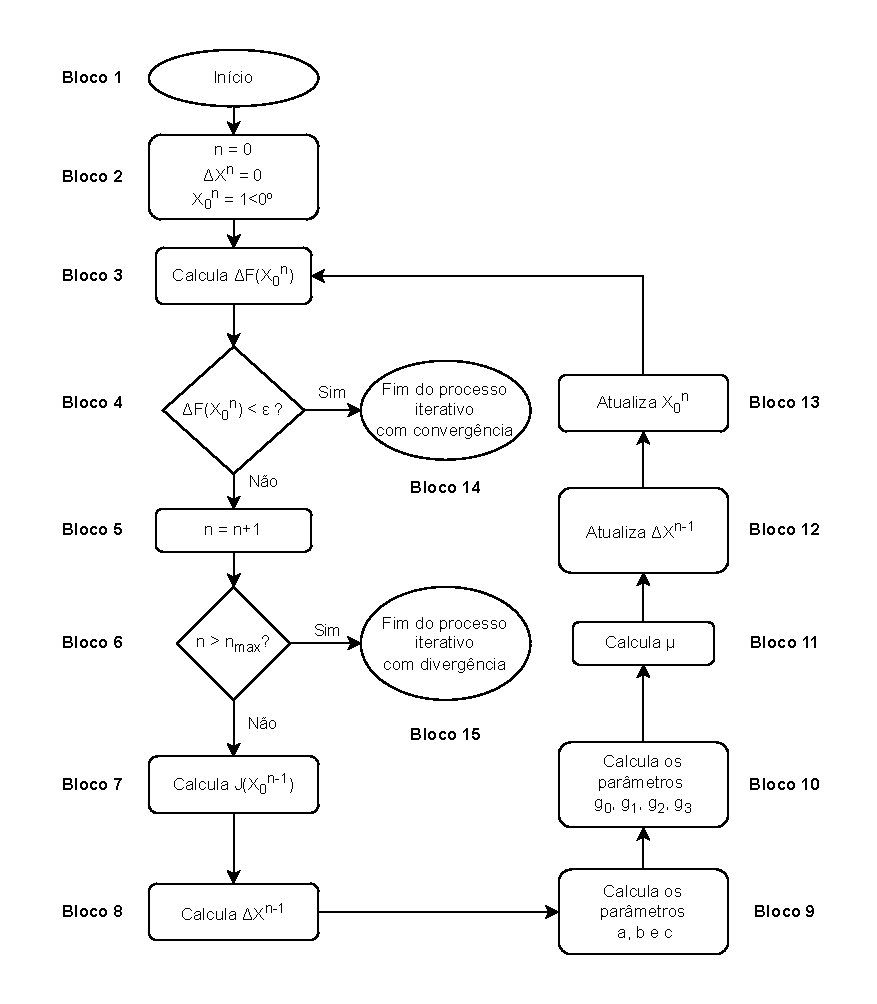
\includegraphics[scale=0.90]{textuais/capitulo3/figuras/Diagrama_NR_OM_5.drawio.pdf}
    \caption*{Fonte: Elaborada pelo autor}
    \label{fig:diagrama_FPOM}
\end{figure}


\section{METODOLOGIA DOS TESTES}
No Capítulo \ref{cap:cap4}, serão apresentados e discutidos os resultados obtidos a partir da aplicação de três variantes apresentadas do método de Newton-Raphson na resolução do problema de \ac{FP}. Os métodos analisados incluem o método em coordenadas retangulares, o método em coordenadas polares e a modificação com Multiplicador Ótimo. O objetivo é comparar a performance e a robustez desses métodos em diferentes cenários, utilizando dois sistemas de teste padrão: o sistema \acs{IEEE} de 14 barras e o sistema \acs{IEEE} de 33 barras. A comparação é realizada com base em 3 testes: carregamento máximo do sistema sem divergência ou soluções espúrias, análise fractal e tempo computacional médio até convergência. 

Todos os experimentos foram realizados em um laptop Acer Nitro 5 com processador Intel Core i5-10300H a 2.50 GHz e 8 GB de RAM, utilizando o sistema operacional Windows 11 Home Single Language, versão 23H2. As simulações foram conduzidas no \textit{software} MATLAB R2021a (9.10.0.1602886). Os testes estão disponíveis no apêndice A.

A metodologia é apresentada a seguir:

\subsection{Carregamento Máximo}
O teste de carregamento máximo visa determinar a fronteira entre a região insolúvel e inviável na situação de aumento sistêmico de carga. O procedimento é detalhado abaixo:
\begin{itemize}
    \item Fator de escala: Definição de um fator de escalonamento $\lambda$ que multiplica as potências ativas e reativas demandadas de todas as barras simultaneamente;
    \item Inicialização: As cargas dos sitemas IEEE 14 e 33 são ajustadas para seus valores base conhecidos, ou $\lambda = 1$, e o erro máximo do \ac{FP} para todas os métodos é definido em  $\epsilon = 10^{-6}$;
    \item Incremento de carga: A carga é aumentada em passos constantes $\Delta \lambda$ até que ocorra a divergência;
    \item Refinamento: Ao detectar divergência, o passo do incremento é reduzido e o fator $\lambda$ é refinado;
    \item Análise: Os fatores de carregamento máximos alcançados por cada método são comparados.
\end{itemize}
\subsection{Análise Fractal}
É conhecido na literatura que as múltiplas soluções do método de \ac{NR} são fractalizadas, isto é, apresentam uma fronteira fractal em sua região de convergência. Isso implica que pequenas variações nas estimativas iniciais próximas à fronteira de convergência podem levar a soluções diferentes do fluxo, como evidenciado por Thorp (\citeyear{thorp}) e Deng et al. (\citeyear{convergence_region}).

Os fractais são construídos plotando-se em um gráfico, onde os eixos representam as variáveis de estado de um problema. Cada par ordenado indica um palpite inicial para o processo e é colorido com base nas diferentes soluções possíveis. Até mesmo pares ordenados que não levam a nenhuma solução podem ser inseridos no mapa em uma determinada cor.

Por isso, plotar os fractais de cada método avaliado pode ser uma ferramenta visual e eficaz capaz de avaliar a robustez do algoritmo considerando sua capacidade de convergência para palpites iniciais diversos. 

Os fractais de Newton para o \ac{FP} teriam uma dimensão igual ao número de variáveis, o que tornaria impossível a representação visual em uma figura \acs{2D}. Uma alternativa é construir um algoritmo que execute diversas combinações de tensão e ângulo como palpites iniciais, mas para todas as barras de forma idêntica. Assim, é possível construir um único fractal \acs{2D} que permitirá a comparação do tamanho da região de convergência dos três métodos.

O teste será conduzido da seguinte forma:
\begin{itemize}
    \item Rodar o \ac{FP} polar, retangular e \ac{FPMO} em carga nominal, média e próxima ao \ac{PMC} com estimativas iniciais de $1\angle 0 ^{\circ}$ e armazenar os valores de tensão e ângulo para cada uma das cargas;
    \item Estabelecer uma faixa de valores que serão iterados os ângulos e fases e rodar o fluxo repetidamente para cada combinação de estimativas iniciais;
    \item Comparar as soluções com a solução previamente calculada;
    \item Se as soluções obedecerem a um erro estabelecido, serão consideradas estáveis; caso contrário, instáveis;
    \item Plotar em um gráfico, utilizando a cor azul para soluções estáveis e vermelho para instáveis;
    \item Analisar as regiões de cada método e compará-las.
\end{itemize}

\subsection{Tempo Computacional e número de iterações}
O teste de tempo computacional visa comparar a eficiência dos métodos em termos de tempo de execução. Medir o tempo necessário para resolver o problema de fluxo de potência é crucial para avaliar o desempenho prático dos algoritmos. Este teste é fundamental para determinar a viabilidade de uma técnica em aplicações de curto prazo, como a operação em tempo real do \ac{SIN}. A descrição da metodologia utilizada está abaixo:

\begin{itemize}
    \item Os algoritmos serão rodados repetidamente nos sistemas teste em carga nominal;
    \item Serão armazenados os tempos e iterações médios do \ac{FP};
    \item Os dados obtidos serão analisados e comparados;
\end{itemize}
\chapter{RESULTADOS E DISCUSSÕES}\label{cap:cap4}  
\section{RESULTADOS PARA O SISTEMA IEEE 33 BARRAS}
O sistema de 33 barras é um padrão de referência amplamente utilizado em estudos de fluxo de potência, planejamento e otimização de redes de distribuição elétrica. Consiste em 33 nós, interconectados por 32 linhas de distribuição, simulando uma rede de distribuição radial. Este sistema é caracterizado por um único ponto de alimentação (barra $V\theta$) e 32 barras de carga (barras $PQ$), representando a distribuição de energia elétrica de uma subestação para diversos consumidores finais. Os dados de barras e de linhas podem ser consultados no apêndice contendo todas as simulações e testes feitos.
\begin{figure}[H]
    \centering
    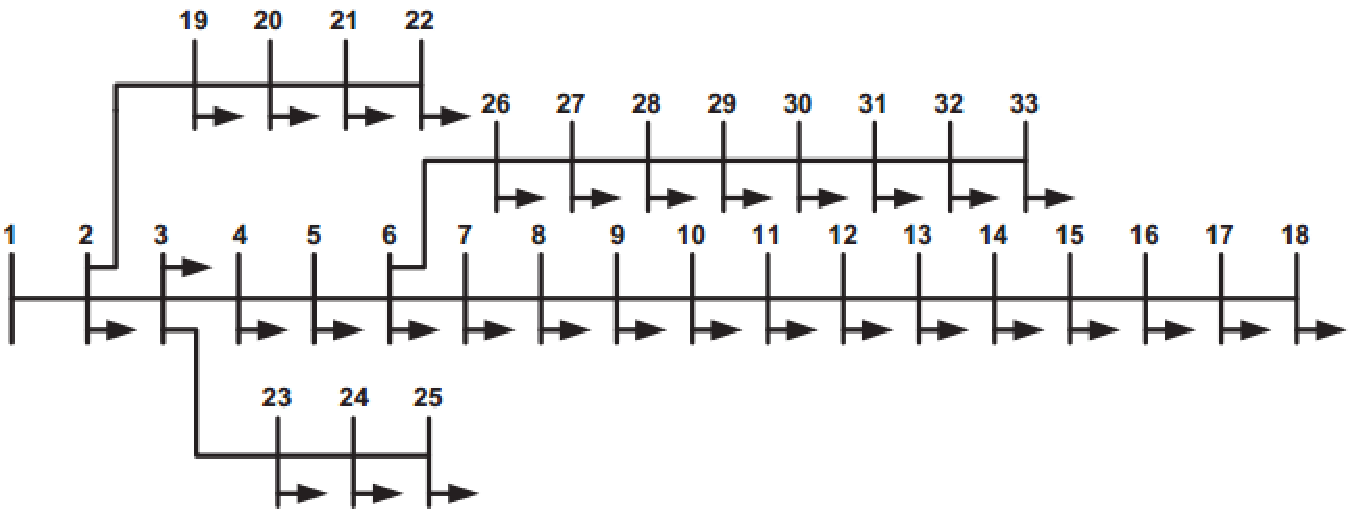
\includegraphics[scale=0.6]{textuais/capitulo4/figuras/IEEE_33BUS.pdf}
    \caption{Topologia do Sistema IEEE 33 Barras}
    \label{fig:14_BUS}
\end{figure}
\subsection{Análise Fractal}
Neste estudo, para obter os mapas fractais que possam ser analisados, foi necessário expandir a faixa de palpites iniciais muito além do usual para um \ac{FP}, indicando que todos os três métodos têm boa capacidade de convergência ao redor de $1 \angle 0^ \circ$. Optou-se pela faixa de $[-0.5, 30]pu$ para o módulo e $[-180, 180]^\circ$ para a fase para uma melhor visualização. Quarenta mil combinações de palpites iniciais foram utilizadas para cada imagem. As seguintes observações foram feitas com os resultados:
\begin{itemize}
    \item As regiões estáveis reduziram de área com o aumento de carga, com exceção do \acs{FPPOL}, que mostrou menor sensibilidade ao $\lambda$;
    \item O Mapa Fractal \acs{FPMO} produziu uma área de convergência muito superior aos outros métodos;
    \item Melhor convergência do \acs{FPRET} e \acs{FPMO} em relação aos ângulos de fase;
    \item Melhor convergência do \acs{FPPOL} em relação ao módulo da tensão;
\end{itemize}



\clearpage
\begin{figure}[H]
    \centering
    \caption{Mapa Fractal FPMO - IEEE 33 Barras}
    \begin{subfigure}[b]{0.45\textwidth}
        \centering
        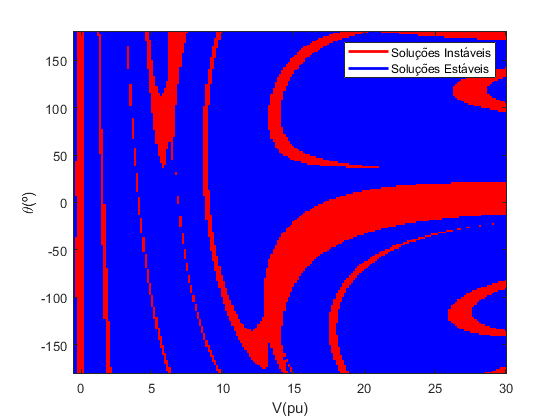
\includegraphics[width=\textwidth]{textuais/capitulo4/figuras/33_FPOM_NOM.png}
        \caption{$\lambda=1$}
    \end{subfigure}
    \vfill
    \begin{subfigure}[b]{0.45\textwidth}
        \centering
        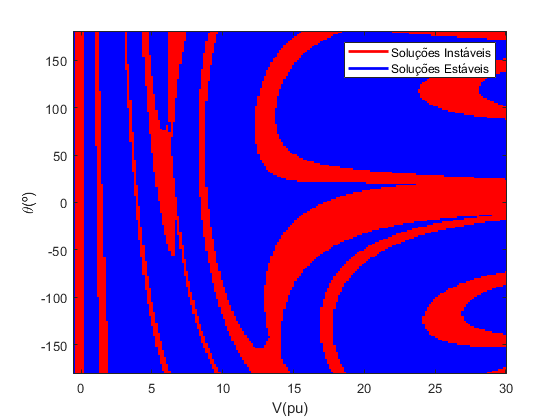
\includegraphics[width=\textwidth]{textuais/capitulo4/figuras/33_FPOM_2lambda.png}
        \caption{$\lambda=2$}
    \end{subfigure}
    \vfill
    \begin{subfigure}[b]{0.45\textwidth}
        \centering
        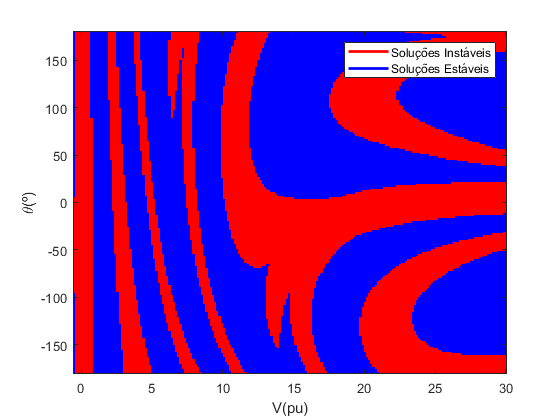
\includegraphics[width=\textwidth]{textuais/capitulo4/figuras/33_FPOM_3lambda.png}
        \caption{$\lambda=3$}
    \end{subfigure}
        \\
   \caption*{Fonte: Elaborada pelo autor}
   \label{fig:FPMO-33}
\end{figure}

\begin{table}[H]
    \centering
    \caption{Área Estável do Mapa Fractal FPMO - IEEE 33 Barras}
    \begin{tabular}{c c c c}
        \toprule
        FPMO & $\lambda = 1$ & $\lambda = 2$ & $\lambda = 3$ \\
        \midrule
        Proporção & $80.99\%$ & $71.89\%$ & $58.24\%$ \\
        \bottomrule
    \end{tabular}
    \caption*{Fonte: Elaborada pelo autor}
    \label{tabela_fractal_FPMO_33}
\end{table}

\clearpage
\begin{figure}[H]
    \centering
    \caption{Mapa Fractal FPPOL - IEEE 33 Barras}
    \begin{subfigure}[b]{0.45\textwidth}
        \centering
        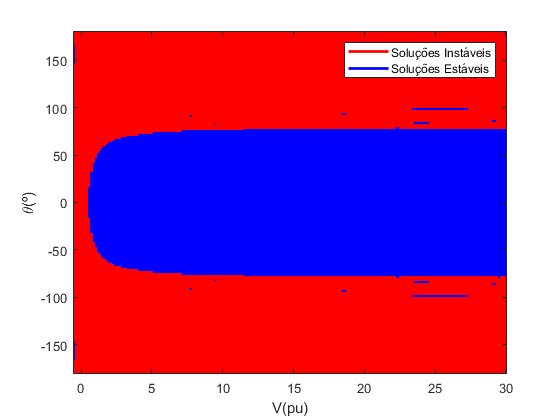
\includegraphics[width=\textwidth]{textuais/capitulo4/figuras/33_FP_POL_NOM.png}
        \caption{$\lambda=1$}
    \end{subfigure}
    \vfill
    \begin{subfigure}[b]{0.45\textwidth}
        \centering
        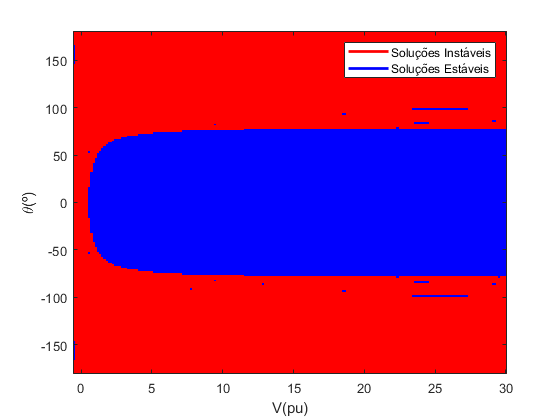
\includegraphics[width=\textwidth]{textuais/capitulo4/figuras/33_FP_POL_2lambda.png}
        \caption{$\lambda=2$}
    \end{subfigure}
    \vfill
    \begin{subfigure}[b]{0.45\textwidth}
        \centering
        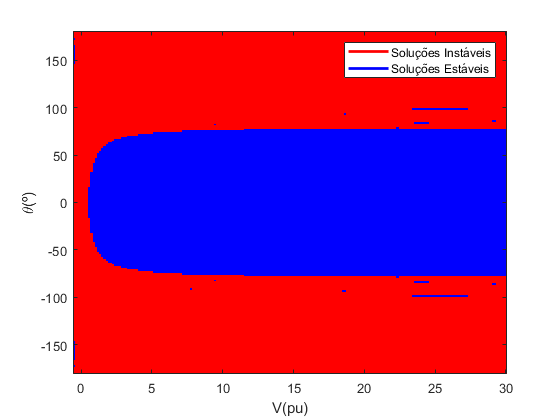
\includegraphics[width=\textwidth]{textuais/capitulo4/figuras/33_FP_POL_3lambda.png}
        \caption{$\lambda=3$}
    \end{subfigure}
        \\
   \caption*{Fonte: Elaborada pelo autor}
   \label{fig:FPPOL-14}
\end{figure}

\begin{table}[H]
    \centering
    \caption{Área Estável do Mapa Fractal FPPOL - IEEE 33 Barras}
    \begin{tabular}{c c c c}
        \toprule
        FPPOL & $\lambda = 1$ & $\lambda = 2$ & $\lambda = 3$ \\
        \midrule
        Proporção & $40.23\%$ & $40.23\%$ & $40.22\%$\\
        \bottomrule
    \end{tabular}
    \caption*{Fonte: Elaborada pelo autor}
    \label{tabela_fractal_FPPOL_33}
\end{table}

\clearpage
\begin{figure}[H]
    \centering
    \caption{Mapa Fractal FPRET - IEEE 33 Barras}
    \begin{subfigure}[b]{0.45\textwidth}
        \centering
        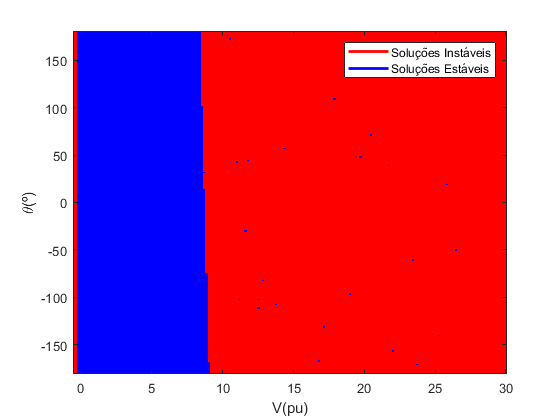
\includegraphics[width=\textwidth]{textuais/capitulo4/figuras/33_FP_RET_NOM.png}
        \caption{$\lambda=1$}
    \end{subfigure}
    \vfill
    \begin{subfigure}[b]{0.45\textwidth}
        \centering
        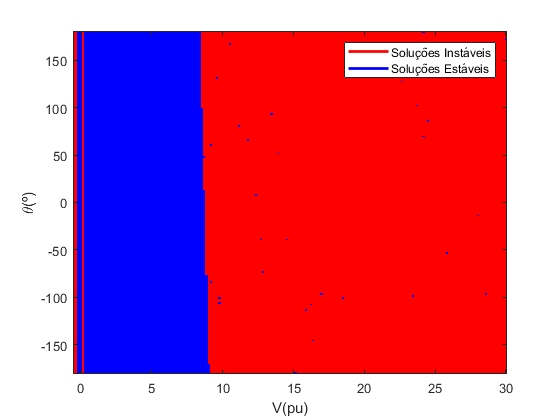
\includegraphics[width=\textwidth]{textuais/capitulo4/figuras/33_FP_RET_2lambda.png}
        \caption{$\lambda=2$}
    \end{subfigure}
    \vfill
    \begin{subfigure}[b]{0.45\textwidth}
        \centering
        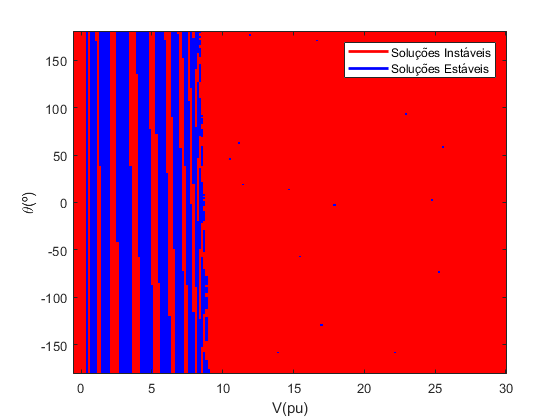
\includegraphics[width=\textwidth]{textuais/capitulo4/figuras/33_FP_RET_3lambda.png}
        \caption{$\lambda=3$}
    \end{subfigure}
        \\
   \caption*{Fonte: Elaborada pelo autor}
   \label{fig:FPRET-33}
\end{figure}

\begin{table}[H]
    \centering
    \caption{Área Estável do Mapa Fractal FPRET - IEEE 33 Barras}
    \begin{tabular}{c c c c}
        \toprule
        FPRET & $\lambda = 1$ & $\lambda = 2$ & $\lambda = 3$ \\
        \midrule
        Proporção & $29.39\%$ & $28.90\%$ & $17.61\%$ \\
        \bottomrule
    \end{tabular}
    \caption*{Fonte: Elaborada pelo autor}
    \label{tabela_fractal_FPRET_33}
\end{table}

\subsection{Tempo Computacional e Número de Iterações}

Foram medidos mil execuções em carga nominal e a média dos tempos computacionais e número de iterações estão registradas na tabela \ref{tabela_tempo_33}.

Constatou-se uma vantagem significante para o método \acs{FPRET} em relação aos outros. Por mais que o \acs{FPMO} tenha tido menor número de iterações, consequência da otimização do próximo passo, seu tempo médio por iteração foi consideravelmente maior, apresentando a pior performance dentre os três métodos.

\begin{table}[H]
    \centering
    \caption{Esforço computacional e iterações - IEEE 33 Barras.}
    \begin{tabular}{c c c }
        \toprule
        Método & Tempo Médio (s)& Número de Iterações Médio \\
        \midrule
        FPMO & 0.0513 & 5 \\
        FPPOL & 0.0389 & 5 \\
        FPRET & 0.0207 & 7 \\
        \bottomrule
    \end{tabular}
    \caption*{Fonte: Elaborada pelo autor}
    \label{tabela_tempo_33}
\end{table}

\subsection{Carregamento Máximo}
Os valores do fator de escala máximo $\lambda$ são apresentados na Tabela \ref{tabela_fatores_escala_33}. Neste caso, foi percebido uma fator de escala maior para o \acs{FPPOL}, seguido do \ac{FPMO} e \ac{FPRET}. 
\begin{table}[H]
\centering
\caption{Fatores de Escala Máximo - IEEE 33 Barras}
\begin{tabular}{c c}
\hline
\textbf{Algoritmo} & \textbf{Fator $\lambda_{max}$} \\
\hline
FPMO &  3.51420 \\
FPPOL & 3.51548 \\
FPRET & 3.51415\\
\hline
\end{tabular}
\label{tabela_fatores_escala_33}
\caption*{Fonte: Elaborada pelo autor}
\end{table}

































\clearpage
\section{RESULTADOS PARA O SISTEMA 14 BARRAS}
O sistema IEEE de 14 barras é um modelo padrão usado para estudos de sistemas de potência, contendo 14 barras, 20 linhas de transmissão, 2 geradores (barras $V\theta$ e $PV$), 3 compensadores síncronos (barras $PV$) e 11 cargas (barras $PQ$). Este sistema representa o sistema elétrico de potência americano da década de 1960. Os dados de barras e de linhas podem ser consultados no apêndice contendo todas as simulações e testes feitos.
\begin{figure}[H]
    \centering
    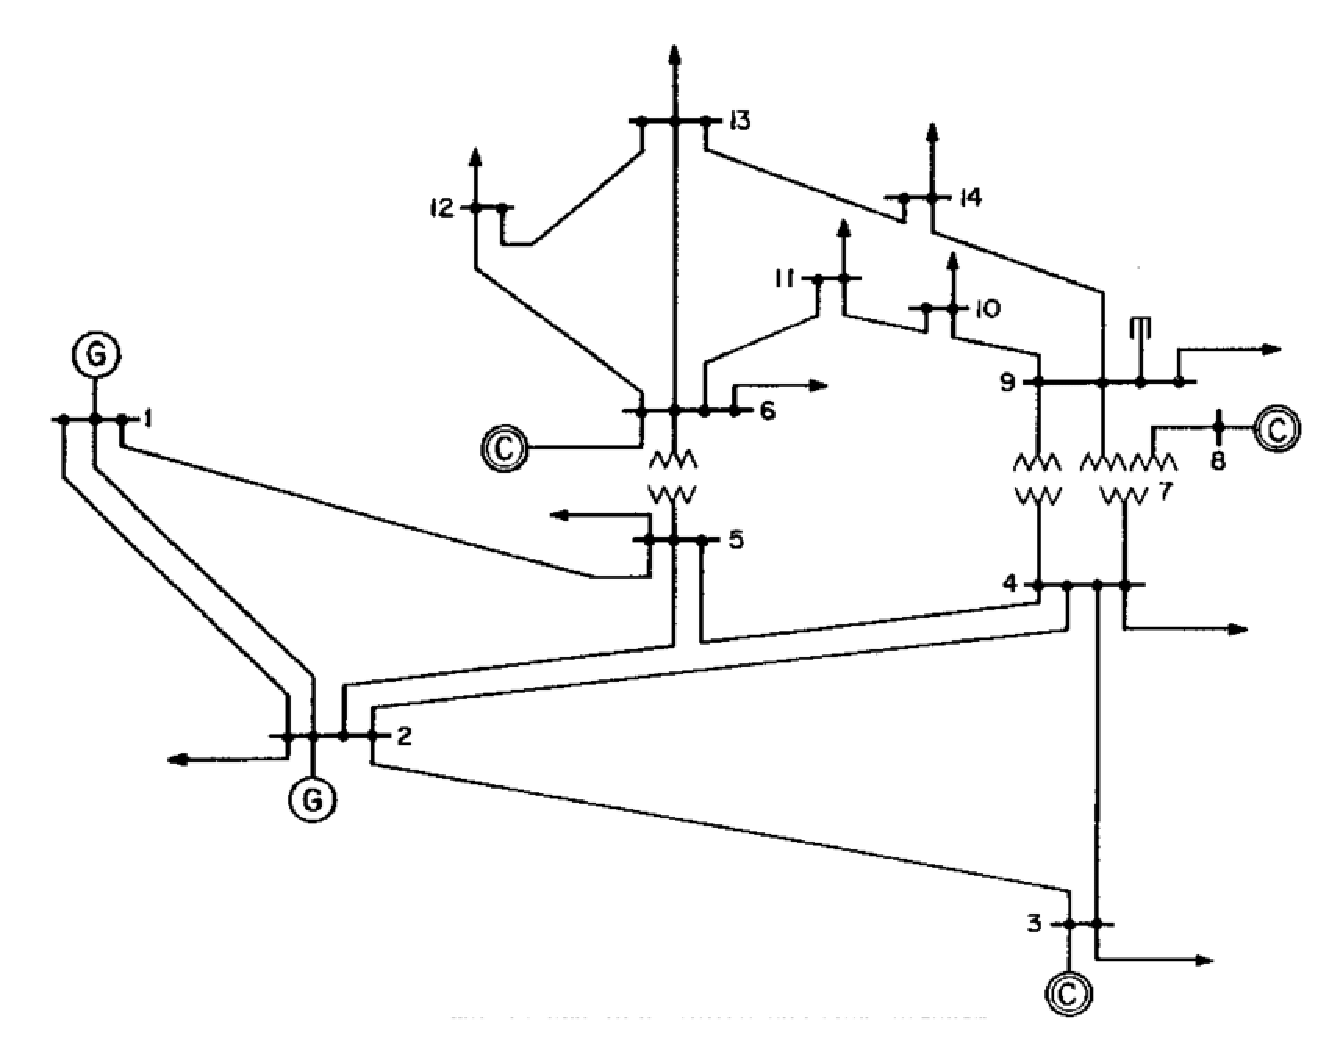
\includegraphics[scale=0.5]{textuais/capitulo4/figuras/IEEE_14BUS.pdf}
    \caption{Topologia do Sistema IEEE 14 Barras}
    \label{fig:enter-label}
\end{figure}

\subsection{Análise Fractal}
Neste sistema também observou-se $100\%$ de região de convergência para a solução do problema ao redor de $1 \angle 0^ \circ$ como palpites iniciais. Da mesma forma que o estudo anterior, optou-se pelo intervalo de $[-0.5, 30]V$ e $[-180, 180]^\circ$ para melhor visualização e comparação dos resultados, além do mesmo número de fluxos rodados por imagem.

\begin{itemize}
    \item As regiões estáveis aumentaram de área com o aumento de carga;
    \item O Mapa Fractal \acs{FPMO} produziu uma área de convergência muito superior aos outros métodos;
    \item Melhor convergência do \acs{FPRET} e \acs{FPMO} em relação aos ângulos de fase como palpites iniciais, maior fraqueza do \acs{FPPOL};
    \item Menor sensibilidade do mapa fractal \acs{FPPOL} com a variação de $\lambda$.
\end{itemize}


\clearpage
\begin{figure}[H]
    \centering
    \caption{Mapa Fractal FPMO - IEEE 14 Barras}
    \begin{subfigure}[b]{0.45\textwidth}
        \centering
        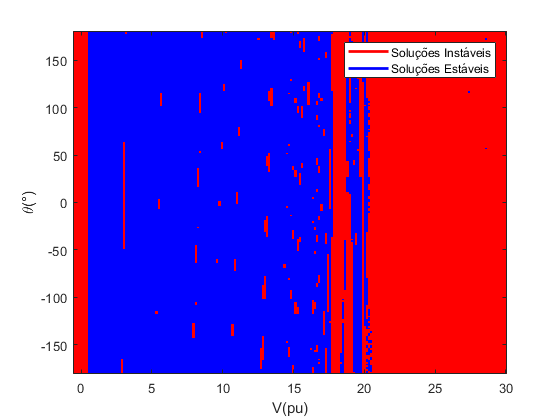
\includegraphics[width=\textwidth]{textuais/capitulo4/figuras/FPOM_nom.png}
        \caption{$\lambda=1$}
    \end{subfigure}
    \vfill
    \begin{subfigure}[b]{0.45\textwidth}
        \centering
        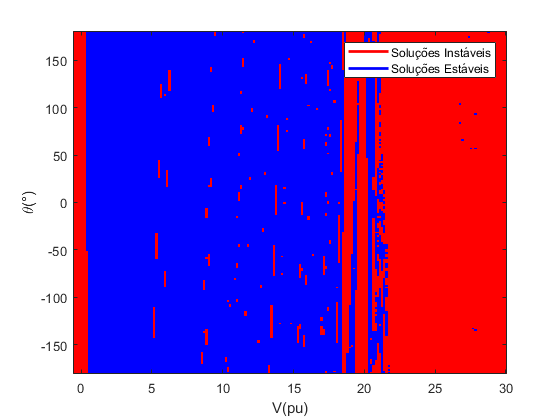
\includegraphics[width=\textwidth]{textuais/capitulo4/figuras/FPOM_10LAMBDA.png}
        \caption{$\lambda=10$}
    \end{subfigure}
    \vfill
    \begin{subfigure}[b]{0.45\textwidth}
        \centering
        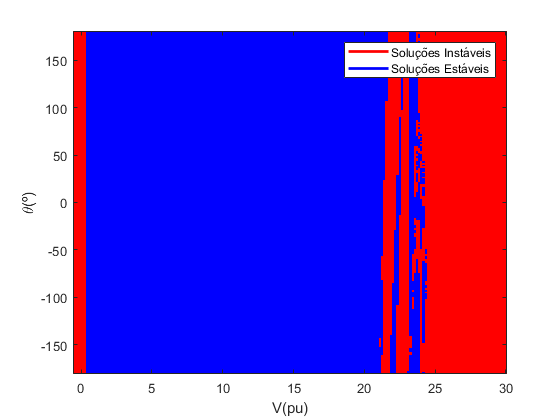
\includegraphics[width=\textwidth]{textuais/capitulo4/figuras/fp_om_20lambda.png}
        \caption{$\lambda=35$}
    \end{subfigure}
        \\
   \caption*{Fonte: Elaborada pelo autor}
   \label{fig:FPMO-14}
\end{figure}

\begin{table}[H]
    \centering
    \caption{Área Estável do Mapa Fractal FPMO - IEEE 14 Barras}
    \begin{tabular}{c c c c}
        \toprule
        FPMO & $\lambda = 1$ & $\lambda = 10$ & $\lambda = 35$ \\
        \midrule
        Proporção & $58.08\%$ & $61.33\%$ & $71.85\%$ \\
        \bottomrule
    \end{tabular}
    \caption*{Fonte: Elaborada pelo autor}
    \label{tabela_fractal_FPMO_14}
\end{table}

\clearpage
\begin{figure}[H]
    \centering
    \caption{Mapa Fractal FPPOL - IEEE 14 Barras}
    \begin{subfigure}[b]{0.45\textwidth}
        \centering
        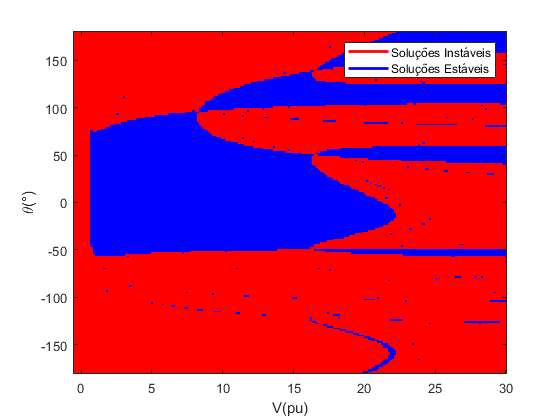
\includegraphics[width=\textwidth]{textuais/capitulo4/figuras/fp_pol_nom.png}
        \caption{$\lambda=1$}
    \end{subfigure}
    \vfill
    \begin{subfigure}[b]{0.45\textwidth}
        \centering
        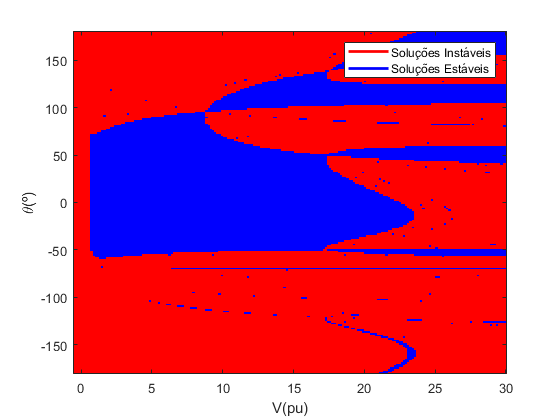
\includegraphics[width=\textwidth]{textuais/capitulo4/figuras/FP_POL_10lambda.png}
        \caption{$\lambda=10$}
    \end{subfigure}
    \vfill
    \begin{subfigure}[b]{0.45\textwidth}
        \centering
        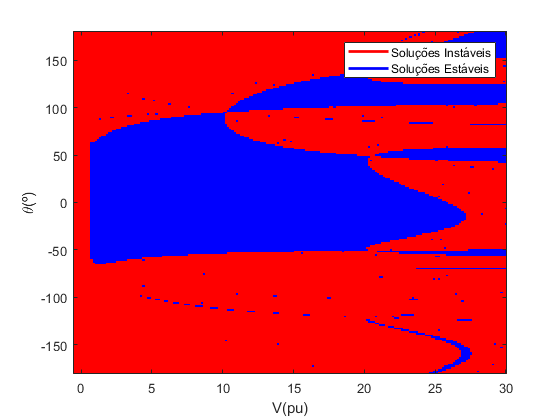
\includegraphics[width=\textwidth]{textuais/capitulo4/figuras/fp_pol_20lambda.png}
        \caption{$\lambda=35$}
    \end{subfigure}
        \\
   \caption*{Fonte: Elaborada pelo autor}
   \label{fig:FPPOL-14}
\end{figure}

\begin{table}[H]
    \centering
    \caption{Área Estável do Mapa Fractal FPPOL - IEEE 14 Barras}
    \begin{tabular}{c c c c}
        \toprule
        FPPOL & $\lambda = 1$ & $\lambda = 10$ & $\lambda = 35$ \\
        \midrule
        Proporção & $30.81\%$ & $31.98\%$ & $33.57\%$\\
        \bottomrule
    \end{tabular}
    \caption*{Fonte: Elaborada pelo autor}
    \label{tabela_fractal_FPPOL_14}
\end{table}

\clearpage
\begin{figure}[H]
    \centering
    \caption{Mapa Fractal FPRET - IEEE 14 Barras}
    \begin{subfigure}[b]{0.45\textwidth}
        \centering
        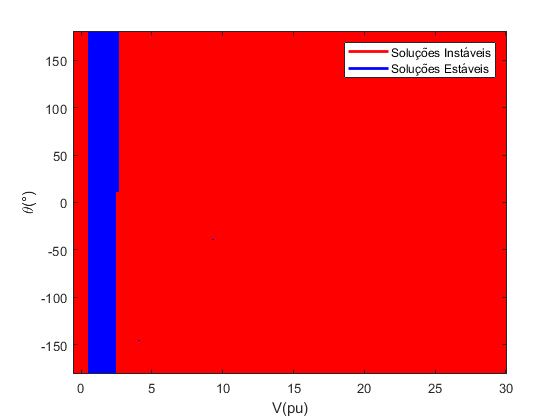
\includegraphics[width=\textwidth]{textuais/capitulo4/figuras/FP_RET_NOM.png}
        \caption{$\lambda=1$}
    \end{subfigure}
    \vfill
    \begin{subfigure}[b]{0.45\textwidth}
        \centering
        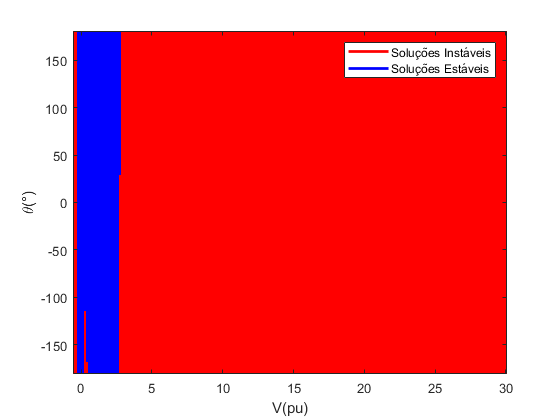
\includegraphics[width=\textwidth]{textuais/capitulo4/figuras/FP_RET_10lambda.png}
        \caption{$\lambda=10$}
    \end{subfigure}
    \vfill
    \begin{subfigure}[b]{0.45\textwidth}
        \centering
        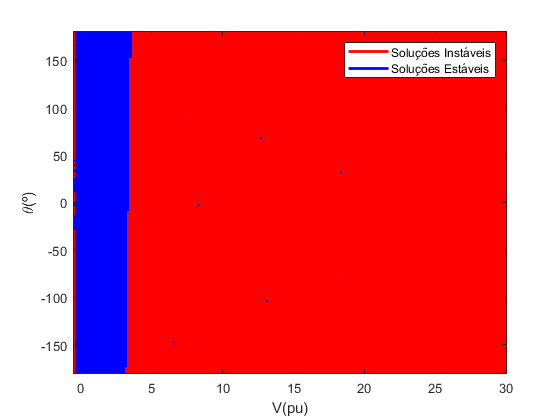
\includegraphics[width=\textwidth]{textuais/capitulo4/figuras/fp_ret_20lambda.png}
        \caption{$\lambda=35$}
    \end{subfigure}
        \\
   \caption*{Fonte: Elaborada pelo autor}
   \label{fig:FPRET-14}
\end{figure}

\begin{table}[H]
    \centering
    \caption{Área Estável do Mapa Fractal FPRET - IEEE 14 Barras}
    \begin{tabular}{c c c c}
        \toprule
        FPRET & $\lambda = 1$ & $\lambda = 10$ & $\lambda = 35$ \\
        \midrule
        Proporção & $6.74\%$ & $9.60\%$ & $12.37\%$ \\
        \bottomrule
    \end{tabular}
    \caption*{Fonte: Elaborada pelo autor}
    \label{tabela_fractal_FPRET_14}
\end{table}


\subsection{Tempo Computacional e Número de Iterações}

Foi observado uma vantagem do \ac{FPRET} em relação a todos os métodos. Nota-se que o \ac{FPMO} reduz o número de iterações médio, mas o tempo adicional de seus cálculos trouxe uma performance geral menor, assim como foi evidenciado para o sistema IEEE 33 Barras.


Na tabela \ref{tabela_tempo_14}, resultado de mil execuções com carregamento nominal, encontram-se os valores de tempo médio e de iterações de cada método para o IEEE 14 Barras. 

\begin{table}[H]
    \centering
    \caption{Esforço computacional e iterações - IEEE 14 Barras.}
    \begin{tabular}{c c c }
        \toprule
        Método & Tempo Médio (s)& Número de Iterações Médio \\
        \midrule
        FPMO & 0.0420 & 6 \\
        FPPOL & 0.0284 & 5 \\
        FPRET & 0.0188 & 7 \\
        \bottomrule
    \end{tabular}
    \caption*{Fonte: Elaborada pelo autor}
    \label{tabela_tempo_14}
\end{table}

\subsection{Carregamento Máximo}
Os valores do fator de escala máximo $\lambda$ são apresentados na Tabela \ref{tabela_fatores_escala_14}. Neste caso, os algoritmos FPRET e FPMO mostraram desempenho praticamente idêntico, apresentando uma diferença a partir da nona casa decimal. Isso indica que ambos os métodos têm uma precisão muito próxima quando sujeitos ao mesmo teste de aumento gradual da carga até a divergência. Em contraste, o método em coordenadas polares obteve um fator de escala ligeiramente menor, indicando uma menor performance comparativa neste cenário específico.


\begin{table}[H]
\centering
\caption{Fatores de Escala Máximo - IEEE 14 Barras}
\begin{tabular}{c c}
\hline
\textbf{Algoritmo} & \textbf{Fator $\lambda_{max}$} \\
\hline
FPMO  & 39.603194459 \\
FPPOL & 38.401057300 \\
FPRET & 39.603194453 \\
\hline
\end{tabular}
\label{tabela_fatores_escala_14}
\caption*{Fonte: Elaborada pelo autor}
\end{table}




\chapter{CONSIDERAÇÕES FINAIS}\label{cap:conclusao}
Ao longo deste estudo, foi avaliada uma modificação do método de Newton-Raphson, o \ac{FPMO}, em relação a outros algoritmos conhecidos na literatura. Pôde-se extrair uma série de conclusões importantes que fornecem perspectivas valiosas para a engenharia elétrica. Ao avaliar o tempo computacional, foi visto que os passos extras tomados para otimizar $\Delta X$ de fato reduziram o número médio de iterações, mas ao custo de aumentar o tempo computacional no geral, sendo o maior ponto negativo do método.

Além disso, verificou-se um ganho marginal no fator de escalonamento máximo $\lambda_{max}$ em relação ao \ac{FPRET}, demonstrando um ganho insignificante de melhoria com os sistemas testes analisados. O \acs{FPPOL} obteve o melhor resultado no IEEE 33 Barras e pior no IEEE 14 Barras, indicando como esse ganho pode variar de sistema para sistema.

Por outro lado, ao analisar os Mapas Fractais \ac{FPMO}, um lado positivo não percebido pelos outros testes foi obtido: um grande aumento na área de convergência em relação ao \ac{FPRET} e \acs{FPPOL}, indicando uma maior robustez numérica. 
Uma vantagem para os algoritmos baseados em coordenadas retangulares foi uma melhor convergência para ângulos de fase variados, porém a fraqueza do \ac{FPRET} para uma maior gama de palpites iniciais para o módulo da tensão foi superada pelo \ac{FPMO}. 

Resumindo, o FPMO apresentou um aumento significativo no tempo computacional e insignificante para $\lambda _{max}$. Seu potencial de melhoria na convergência numérica, evidenciado pelos Mapas Fractais, sugere que esse método de fato traz melhorias na robustez numérica. No entanto, para o problema específico do \ac{FP}, isso não foi aplicável, pois a boa escolha da aproximação inicial (próximo de $1\angle 0^\circ$) já garante uma convergência rápida e eficiente com métodos tradicionais. Portanto, embora o \ac{FPMO} ofereça vantagens teóricas, sua aplicabilidade prática para o problema em questão se provou ineficiente nos sistemas analisados devido ao aumento do esforço computacional e à eficácia já alcançada com métodos existentes. 


\section{DIRETRIZES PARA TRABALHOS FUTUROS}

Destaca-se como possíveis trabalhos futuros a serem abordados em outras pesquisas:\vspace{-1em}
\begin{itemize}
    \item Avaliação da dimensão Haussdorf dos fractais de diferentes métodos numéricos para \ac{FP}, podendo indicar alguma mensuração da estabilidade numérica;
    \item Analisar os mapas fractais do \ac{FPMO} na formulação por injeção de correntes, que é mais rápida;
    \item Entender por que diferentes sistemas podem reduzir ou aumentar a região de convergência com o aumento de carga com o mesmo algoritmo utilizado;
    \item Analisar a viabilidade do \ac{FPMO} diretamente em coordenadas polares e para sistemas mal condicionados;
    \item Explorar a análise fractal em sistemas mais complexos com controles de tensão e reativos.
\end{itemize}

%% ----------------------------------------------------------

%% ELEMENTOS POS-TEXTUAIS

%\postextual 

%% Bibliografia
\bibliography{./bibliografia}  % o nome do arquivo .bib com as referências

% Apendices
\begin{apendicesenv}
\chapter{Implementações Computacionais}\label{cap:ApendiceA}

A seguir, é disponibilizado o link que contém todos os códigos computacionais implementados em \textit{MATLAB} durante a execução deste estudo. 
\Urlmuskip=0mu plus 1mu
\def\UrlBreaks{\do\/\do-}

Disponível em : \url{https://l1nk.dev/5za0p}

\end{apendicesenv}

%%% ---
\end{document}

%%%%EXEMPLO QUANDO SE TEM TODAS AS ILUSTRA\c{C}\~OES DO MESMO TIPO. POR EXEMPLO, ORGANOGRAMA.

%No meio do texto acima, localize o comando \pdfbookmark[0]{\listfigurename}{lof} . Ap\'os ele e antes do comando \listoffigures* , retire os 
%comandos (ou coloque % no in\'icio da linha deles) \ilustvaria e \listilustvaria . Acrescente os dois comandos abaixo 

\tipoilust{Fotografia} %Preencha com o tipo de sua ilustra\c{c}\~ao (somente caso todas sejam do mesmo tipo). Por exemplo, Organograma.
\renewcommand{\listfigurename}{\textbf{LISTA DE FOTOGRAFIAS}} %Troque ORGANOGRAMAS por outra palavra conforme o tipo de sua ilustra\c{c}\~ao, se for \'unico.

%e retire % do in\'icio do comando abaixo
\listoffigures* %Use este comando quando todas as ilustra\c{c}\~oes s\~ao do mesmo tipo e caso queira inserir a lista delas.

%Exemplo para se colocar a ilustrac\{c}\~ao neste caso, de tipo \'unico (por exemplo, Organograma) em todo o trabalho.
\begin{figure}[h]
\larguratexto{6cm}  %mesma largura da ilustra\c{c}\~ao, dada em ``[width=6cm]'' abaixo
\begin{center}
\caption{Logotipo da UFJF} %Informa\c{c}\~ao acima da figura
\includegraphics[width=6cm]{logo.jpg}
\fonte{Universidade Federal de Juiz de Fora (2012).} %Indicar a fonte consultada (elemento obrigat\'orio, mesmo que seja produ\c{c}\~ao do pr\'oprio autor).
\end{center}
\end{figure}



